%%\documentclass{../doc/tex/lifestyle}
\documentclass[a4paper]{book}
%\documentclass{article}

\usepackage{a4wide}
\usepackage[utf8]{inputenc}
\usepackage[T1]{fontenc}
\usepackage{svninfo}
%%\usepackage{fullpage}
\usepackage{longtable}

\usepackage{url}
\usepackage{fancyhdr}
\pagestyle{fancyplain}
\fancyhead[RE,LO]{\leftmark}
\fancyhead[LE,RO]{\thepage}

\usepackage{fancybox}
%\usepackage{fancyvrb}
%\usepackage{color}
\usepackage{xspace}
\usepackage{multicol}
\usepackage{makeidx}
\usepackage{subfigure}
\usepackage{verbatim}

\usepackage[english]{babel}
\usepackage{tabularx}

\usepackage{subfigure}
\usepackage{graphicx}
\graphicspath{%
  {pdfs/}%
  {pngs/}
}
\usepackage{amsmath,amssymb}

\usepackage{xspace,pgf,pgfkeys,pgfmath}
\usepackage{tikz}
\usetikzlibrary{arrows,patterns,plotmarks,shapes,snakes,er,3d,automata,backgrounds,topaths,trees,petri,mindmap}

%
% les trois parties (front, main et back)
%

\renewcommand\backmatter{%
%  \let\minisommaire\null
  \cleardoublepage
 % \@mainmatterfalse
 % \@frontmatterfalse
  \fancyfoot{}
  \fancyhead[LE]{\bfseries\thepage}
  \fancyhead[RO]{\bfseries\thepage}
  \fancyhead[LO]{\bfseries\rightmark}
  \fancyhead[RE]{\bfseries\leftmark}
 % \renewcommand{\toclevel@chapter}{-1}% pour avoir le bookmark au même niveau
 %                                     % que part
}









%-----------------------------------------------------------------------
% index
\usepackage{index}
%-----------------------------------------------------------------------
%
% espace verticale entre les groupes dans l'index
%
\renewcommand\indexspace{\par \vskip 20pt plus5pt minus3pt\relax}
%-----------------------------------------------------------------------


%-----------------------------------------------------------------------
%
% pour avoir un lien correct dans les bookmark du pdf, sur l'index
%
\let\printindexORIG\printindex
\renewcommand{\printindex}{%
  \cleardoublepage
  \phantomsection% création d'une fausse section
  \addcontentsline{toc}{chapter}{Index}
  \printindexORIG}


\AtBeginDocument{%
  \makeindex%
}

%-----------------------------------------------------------------------


%-----------------------------------------------------------------------
% fancyvrb unixcom environment
\usepackage{styles/fvrb}

%-----------------------------------------------------------------------
% nota environment
\usepackage{styles/nota}
\newcommand{\ficnota}{attention}
\newcommand{\ficnote}{note}
\newcommand{\ficnotahack}{question}

\setlength{\largeurnota}{.8cm}
\newenvironment{nota}{%
  \begin{pictonote}{\ficnota}}{\end{pictonote}}
\newenvironment{note}{%
  \begin{pictonote}{\ficnote}}{\end{pictonote}}
\newenvironment{notahack}{%
  \begin{pictonote}{\ficnotahack}}{\end{pictonote}}


\usepackage{xcolor}
\newtheorem{problem}{Problem}



\definecolor{lbcolor}{rgb}{0.95,0.95,0.95}
\definecolor{cblue}{rgb}{0.,0.0,0.6}

\usepackage[colorlinks=true]{hyperref}
\usepackage{filecontents,listings}
\lstset{language=c++,showspaces=false,showstringspaces=false,captionpos=t,literate={>>}{\ensuremath{>>}}1}
%\lstset{float}
\lstset{basicstyle=\small\ttfamily}
\lstset{lineskip=-2pt}
\lstset{keywordstyle=\color{red}\bfseries}
%\lstset{keywordstyle=\mdseries\color{red}}
\lstset{emph={inline},emphstyle=\color{red}\bfseries}
%\lstset{stringstyle=\ttfamily}
\lstset{commentstyle=\ttfamily\color{cblue}}
\lstset{backgroundcolor=\color{lbcolor},rulecolor=}
%\lstset{numbers=left}
%\lstset{numbers={none}}
%\lstset{numberstyle=\tiny}
%\lstset{numbersep=1pt}
\lstset{frame=single,framerule=0.5pt}
\lstset{belowskip=\smallskipamount}
\lstset{aboveskip=\smallskipamount}
\lstset{emph={constant,cst,cst_ref,constant_ref,val,integrate,on,grad,gradt,gradv,dot,id,dx,dy,dz,idt,dxt,dyt,dzt,div,divt,idv,dxv,dyv,dzv,dn,dnt,mass,stiffness,trans,trace,jump,jumpt,average,averaget,maxface,project,P,Px,Py,Pz,h,H,Hface,hFace,N,Nx,Ny,Nz,sqrt,sin,cos,min,max,abs,sign,pow,chi,exp,log,form1,form2, FunctionSpace, bases,
prod,element_prod, range, subrange, inner_prod,unite,elements,markedelements,markedfaces,boundaryfaces,_Q},emphstyle=\color{blue}}
\lstset{includerangemarker=false,rangeprefix=\/\/\#\ ,% curly left brace plus space
  rangesuffix=\ \#}% space plus curly right brace

\newcommand{\acos}{\ensuremath{\mathrm{acos}}\xspace}
\newcommand{\asin}{\ensuremath{\mathrm{asin}}\xspace}
\newcommand{\atan}{\ensuremath{\mathrm{atan}}\xspace}
%\newcommand{\tanh}{\ensuremath{\mathrm{tanh}}\xspace}
\newcommand{\cpp}{C{\hspace{-.3em}\vspace{-.2em}\tiny++}\xspace}
\newcommand{\nel}{{\ensuremath{N_{\text{el}}}}}
\newcommand{\polyP}[1]{\ensuremath{\mathbb{P}_{#1}}\xspace}
\newcommand{\life}{Life\xspace}
\newcommand{\cmake}{\texttt{cmake}\xspace}
\newcommand{\ccmake}{\texttt{ccmake}\xspace}

\InputIfFileExists{version}{}{\def\lifeversion{\texttt{x.y.z}}}
\title{Life Manual\\
A Library for Finite and Spectral Element Methods in 1D, 2D and 3D\\
{\small \lifeversion }}
\author{Christophe Prud'homme\thanks{Université de Grenoble,
51, rue des Mathématiques, BP53,38041 Grenoble}}
\date{\svnToday}

\thispagestyle{empty}
\begin{document}
\thispagestyle{empty}
\svnInfo $Id$


% \CssFile
% /* css.sty */
% body { width: 75% }
% h1,h2,h3,h4,h5,h6,pre,code,p {font-size: 1em; font-weight: normal; }
% dl,li,dt,dd,h1,h2,h3,h4,h5,h6,pre,form,body,html,p,blockquote,fieldset,input {margin: 0; padding: 0;}
% h2,h3,h4,h5,h6 { color: #B30000; }
% h1 { color: #FFB267; }
% h2 { border-bottom: 1px dotted #FFB267; border-left: 1px dotted #FFB267; }
% h3 { border-bottom: 1px dotted #D95934; }

% div.lstlisting{background: #eee; border: thin solid #000;  }
% div.lstinputlisting{background: #eee; border: thin solid #000; }

% \EndCssFile

%\maketitle

\begin{center}
  {\Large
    LIFE MANUAL\\
    A LIBRARY FOR \\
    FINITE AND SPECTRAL ELEMENT METHODS IN\\
    1D, 2D AND 3D\\
    {\small \lifeversion }}\\[0.6cm]
  Christophe \textsc{Prud'homme}\\
  \texttt{christophe.prudhomme@ujf-grenoble.fr}\\
  \par\vspace{2cm}

  \begin{flushright}
    \footnotesize
    Version du \svnInfoDate\\
    Revision \svnInfoRevision
  \end{flushright}
  \par\vspace{5cm}

  \centerline{\begin{minipage}[l]{0.35\linewidth}
    
\includegraphics[width=.7\linewidth]{logo-ujf}
  \end{minipage}
  \begin{minipage}[r]{0.35\linewidth}
    
\includegraphics[width=.7\linewidth]{logo-ljk}
  \end{minipage}}


\end{center}

\vfill \mbox{} \clearpage

\thispagestyle{empty}


\vfill
Permission is granted to copy, distribute and/or modify this document
under the terms of the GNU Free Documentation License, Version 1.2
or any later version published by the Free Software Foundation;
with no Invariant Sections, no Front-Cover Texts, and no Back-Cover Texts.
A copy of the license is included in the section entitled "GNU
Free Documentation License".

\newpage

\tableofcontents

\chapter{Building and Programming Environment}


\section{Building Life}

\subsection{Getting the source via an archive}
\label{sec:getting-source-via-1}

\life is distributed as a tarball once in a while. The tarballs are available
at
\begin{center}
  \href{http://ljkforge.imag.fr/life}{http://ljkforge.imag.fr/life}
\end{center}
Download the latest tarball. Then follow the steps and replace
\texttt{x},\texttt{y},\texttt{z} with the corresponding numbers

\begin{unixcom}
  tar xzf life-x.y.z.tar.gz
  cd life-x.y.z
\end{unixcom}


\subsection{Getting the source via Subversion}
\label{sec:getting-source-via}

\paragraph{Creating RSA keys}
\label{sec:creation-rsa-keys}
In order to download the sources of \life, you have to go in
LJKForge website (https://ljkforge.imag.fr) and create an account. After the
administrator approval, you have to demand the rights to see the project tree.

Then, you will have to create RSA keys to be able to connect to the server
using ssh. To do that you have to type the commands :
\verb|ssh-keygen -t dsa| and \linebreak[2] \verb|ssh-keygen -t rsa| to create
the keys. After that, you have to copy the \verb|id_dsa.pub| and
\verb|id_rsa.pub| files in the My Page > Account Maintenance > Edit SSH Keys
section of the LJKForge website. Those files are located in the \verb|~/.ssh/|
folder of your computer. You will be able to connect to the server within an
hour.
\\
{\bfseries Important : } If you don't have the same login on your computer as on
LJKForge, you must add the commands
\begin{lstlisting}[language=sh]
host ljkforge.imag.fr
  user <your_login_ljkforge>
\end{lstlisting}
in the \verb|~/.ssh/config| file.

\subsubsection{Downloading the sources}
\label{sec:download-sources}

To be able to download the \life sources, you need subversion and SSH > 1.xxx
installed on your computer. In a command prompt, go where you want \life to be
downloaded and type the following command.
\\ \verb|svn co svn+ssh://login@ljkforge.imag.fr/svn/life/life/trunk life|
where \\ \verb|login| is your login name in the LJKForge plateform. Then, if
you want to download the life-test sources type :
\begin{unixcom}
  cd life/benchmarks
  svn co svn+ssh://login@ljkforge.imag.fr/svn/life-test/life-test/trunk validation
\end{unixcom}

\subsection{Dealing with software dependencies}
\label{sec:about-dependencies}

In order to install \life, you have to install many dependencies
before. Those libraries and programs are necessary for the
compilation and installation of the \life librairies.

This is the list of all the librairies you must have installed on your
computer, and the \verb|*-dev| packages for some of them.

Here is the list of required packages:
\begin{itemize}
\item g++ (>=4.1)
\item MPI : openmpi (preferred) or mpich
\item Boost (>=1.37)
\item Petsc (>=2.3.3)
\item autoconf, automake, libtool (required in subversion mode)
\item Gmsh\footnote{Gmsh is a pre/post processing software for scientific
computing available at \url{http://www.geuz.org/gmsh}}
\item Libxml2
\end{itemize}

Here is the list of optional packages:
\begin{itemize}
\item Eigen2
\item Superlu
\item Suitesparse(umfpack)
\item Metis: scoth with the metis interface (preferred), metis (non-free)
\item Trilinos (>=8.0.8)
\item Google perftools
\item Paraview\footnote{Paraview is a few parallel scientific data
    visualisation plateform, \url{http://www.paraview.org}}, this is
  not stricly required to run \life programs but it is somehow
  necessary for visualisation
\item Python (>= 2.5) for the validation tools
\end{itemize}

Note that all these packages are available under Debian/GNU/Linux and
Ubuntu. They should be available

\subsection{Compiling Life with the CMake}

Life build system supports
\cmake\index{cmake}\footnote{\url{http://www.cmake.org}}. This should become the
preferred way to build \life as it is much simpler and more powerful in many
ways than the autotools.

\life, using \cmake, can be built either in source and out of source and different
build type:
\begin{itemize}
\item minsizerel : minimal size release
\item release release
\item debug : debug
\item none(default)
\end{itemize}

\paragraph{CMake In Source Build}

Enter the source tree and type
\begin{unixcom}
  cmake .
  make
\end{unixcom}

To customize or change some build setting one can use the \cmake curse interface
\ccmake
\begin{unixcom}
  ccmake . # configure and generate
  make
\end{unixcom}

\paragraph{CMake Out Source Build}

Create a build directory

\subsection{Compiling Life with the AutoTools}

Go in the same folder in wich you have done the checkout and type the following
commands :

\subsubsection{From tarball}
\label{sec:from-tarball}

The steps are as follows to configure the \life Development Plateform

\begin{unixcom}
  cd life-x.y.z
  mkdir opt
  cd opt

  ../configure --enable-opt2
\end{unixcom}

Then type
\begin{unixcom}
  make
\end{unixcom}

to compile the library and the tutorial. And finally type
\begin{unixcom}
  make check
\end{unixcom}
In order to compile the testsuite, the examples and the benchmarks and
execute some of them to verity that the \life library is functional.


\subsubsection{From subversion}
\label{sec:from-subversion}

The steps are as follows to configure the \life Development Plateform

\begin{unixcom}
  cd life
  make -f Makefile.dist
  mkdir opt
  cd opt

  ../configure --enable-opt2
\end{unixcom}

Then, to build  the \life library, type
\begin{unixcom}
  make
\end{unixcom}

And finally to check the library, type
\begin{unixcom}
  make check
\end{unixcom}


\begin{note}
  The script \lstinline!configure! supports many command line
  options. In particular if you are interested in writing some code or
  examples inside the \life environment you have to enable the so
  called \emph{maintainer mode} to ensure that the makefiles are
  properly regenerated when you modify a \lstinline!Makefile.am! or if
  you modify \lstinline!configure.ac!, to achieve this type
  \begin{unixcom}
    configure --enable-maintainer-mode
  \end{unixcom}
  To list all configure options, type
  \begin{unixcom}
    configure --help
  \end{unixcom}
\end{note}


\subsubsection{Compiling an extra module}
\label{sec:compile-an-extra}

If you work with an extra module, \emph{e.g.} \lstinline!validation!, the steps are as follows
\begin{unixcom}
cd life
make -f Makefile.dist
cd benchmarks/validation
make -f Makefile.dist
cd ../../..
mkdir opt
cd opt
../life/configure --enable-opt2 --enable-maintainer-mode
make
make check
\end{unixcom}


\subsubsection{Compiling the Life tutorial}
\label{sec:comp-life-tutor}
If the command \lstinline!make check! has been run before the tutorial
should be already compiled and ready. The steps are as follows  to build the Life tutorial
\begin{unixcom}
  cd opt/doc/tutorial
  make check
\end{unixcom}
Here is what the directory should look like
\begin{unixcom}
  cd opt/doc/tutorial
  ls

  laplacian     Makefile      myintegrals   mymesh       pngs/
  tutorial.blg  tutorial.out  tutorial.toc  laplacian.o  myapp
  myintegrals.o mymesh.o      stokes.assert tutorial.aux pdfs/ styles/
  stokes        stokes.o      tutorial.bbl  tutorial.log tutorial.pdf
\end{unixcom}


\section{Programming environment}

\section{Namepaces}

\begin{itemize}
\item \lstinline!Life!
\item \lstinline!Life::po!
\item \lstinline!Life::mpl!
\item \lstinline!Life::ublas!
\item \lstinline!Life::math!
\item \lstinline!Life::fem!
\item \lstinline!Life::vf!

\end{itemize}

\section{Libraries}

\begin{itemize}
\item \lstinline!life/lifecore!
\item \lstinline!life/lifealg!
\item \lstinline!life/lifepoly!
\item \lstinline!life/lifediscr!
\item \lstinline!life/lifefilters!
\item \lstinline!life/lifevf!
\end{itemize}

\chapter{Tutorial}
\label{sec:tutorial}


\section{Creating applications}
\label{sec:creat-appl}


\marginpar{\lstinline!myapp.cpp!}

\subsection{Application and Options}
\label{sec:options}

As a \life user, the first step in order to use \life is to create an
application. First we include the \lstinline!Application! header file,
\lstinline!life/lifecore/application.hpp! and the header which the
internal \life options. \life uses the
\lstinline!boost::program_options!\footnote{\url{http://www.boost.org/doc/html/program_options.html}}
library from Boost to handle its command line options


\lstinputlisting[linerange=marker1-endmarker1]{myapp.cpp}

Next to ease the programming and reading, we use the \lstinline!using!
\cpp directive to bring the namespace Life to the current namespace

\begin{lstlisting}
  using namespace Life;
\end{lstlisting}

Then we define the command line options that the applications will
provide. Note that on the \lstinline!return! line, we incorporate the
options defined internally in \life.

\lstinputlisting[linerange=marker2-endmarker2]{myapp.cpp}

In the example, we provide the options \lstinline!dt! which takes an
argument, a \lstinline!double! and its default value is \lstinline!1!
if the options is not set by the command line.

Then we describe the application by defining a class
\lstinline!AboutData! which will be typically used by the
\lstinline!help! command line options to describe the application


\lstinputlisting[linerange=marker3-endmarker3]{myapp.cpp}


Now we turn to the class \lstinline!MyApp! itself: it derives from
\lstinline!Life::Application!. Two constructors take \lstinline!argc!,
\lstinline!argv! and the \lstinline!AboutData! as well as possibly the
description of the command line options \lstinline!Life::po::option_description!.

The class \lstinline!MyApp! must redefine the \lstinline!run()! member
function. It is defined as a pure virtual function in
\lstinline!Application!.


\lstinputlisting[linerange=marker4-endmarker4]{myapp.cpp}

The implementation of the constructors is usually simple, we pass the
arguments to the super class \lstinline!Application! that will analyze
them and subsequently provide them with a
\lstinline!Life::po::variable_map! data structure which operates like
a \lstinline!map!. Have a look at the document
\lstinline!boost::program_options! for further details.

\lstinputlisting[linerange=marker5-endmarker5]{myapp.cpp}

The \lstinline!run()! member function holds the application
commands/statements. Here we provide the smallest code unit: we print
the description of the application if the \lstinline!--help! command
line options is set.

\lstinputlisting[linerange=marker6-endmarker6]{myapp.cpp}

Finally the \lstinline!main()! function can be implemented. We pass
the results of the \lstinline!makeAbout()! and
\lstinline!makeOptions()! to the constructor of \lstinline!MyApp! as
well as \lstinline!argc! and \lstinline!argv!. Then we call the
\lstinline!run()! member function to execute the application.

\lstinputlisting[linerange=marker7-endmarker7]{myapp.cpp}

After compiling \lstinline!myapp!, we can execute it

\begin{lstlisting}[language=sh]
> myapp --help
myapp: my first Life application
Allowed options:

MyApp options:
  --dt arg (=1)                              time step value

>./myapp --authors
myapp: my first Life application
          Author Name       Task                          Email Address
-----------------------------------------------------------------------
Christophe Prud'homme   developer  christophe.prudhomme@ujf-grenoble.fr
\end{lstlisting}

\subsection{Application, Logging and Archiving}
\label{sec:appl-logg-arch}

\life provides some basic logging and archiving support: using the
\lstinline!changeRepository! member functions of the class
\lstinline!Application!, the logfile and results of the application
will be stored in a subdirectory of \lstinline!~/life!. For
example the following code

\lstinputlisting[linerange=marker8-endmarker8]{myapp.cpp}

will create the directory \lstinline!~/life/myapp! and will store the
logfile and any files created after calling
\lstinline!changeRepository!. Refer to the documentation of
\lstinline!Boost::format! of further details about the arguments to be
passed to \lstinline!changeRepository!. The logfile is named
\lstinline!~/life/myapp/myapp-1.0!. The name of the logfile is built
using the application name, here \lstinline!myapp!, the number of
processes, here 1 and the id of the current process, here 0.

\begin{lstlisting}[language=sh]
> myapp
> cat ~/life/myapp/myapp-1.0
myapp-1.0 is opened for debug
[Area 0] the value of dt is 1

> myapp --dt=0.1
> cat ~/life/myapp/myapp-1.0
myapp-1.0 is opened for debug
[Area 0] the value of dt is 0.1
\end{lstlisting}

\subsection{MPI Application}

\marginpar{\lstinline!myapp.cpp!}
\life relies on MPI for parallel computations and the class
\lstinline!Application!  initialises the MPI environment.

\begin{lstlisting}[language=sh]
> mpirun -np 2 mympiapp
> cat ~/life/mympiapp/mympiapp-2.0
mympiapp-2.0 is opened for debug
[Area 0] the value of dt is 1
[Area 0] we are on processor eta
[Area 0] this is process number 0 out of 2
> cat ~/life/mympiapp/mympiapp-2.1
mympiapp-2.1 is opened for debug
[Area 0] the value of dt is 1
[Area 0] we are on processor eta
[Area 0] this is process number 1 out of 2

> mpirun -np 2 mympiapp --dt=0.01
> cat ~/life/mympiapp/mympiapp-2.0
mympiapp-2.0 is opened for debug
[Area 0] the value of dt is 0.01
[Area 0] we are on processor eta
[Area 0] this is process number 0 out of 2
> cat ~/life/mympiapp/mympiapp-2.1
mympiapp-2.1 is opened for debug
[Area 0] the value of dt is 0.01
[Area 0] we are on processor eta
[Area 0] this is process number 1 out of 2
\end{lstlisting}

\subsection{Initializing PETSc and Trilinos}

\index{PETSc}\index{Trilinos}\index{Libraries!PETSc}\index{Libraries!Trilinos}

\life supports also the PETSc and Trilinos framework, the class
\lstinline!Application!\index{Class!Application} takes care of
initialize the associated environments.

\section{Mesh Manipulation}
\label{sec:mesh-manipulation}

\index{mesh}\index{Class!Mesh}
\marginpar{\lstinline!mymesh.cpp!}
In this section, we present some of the mesh definition and
manipulation tools provided by \life.

\subsection{Mesh definition}

We look at the definition of a mesh data structure. First, we define
the type of geometric entities that we shall use to form our mesh. \life supports
\begin{itemize}
\item simplices: segment, triangle, tetrahedron
\item tensorized entities: segment, quadrangle, hexahedron
\end{itemize}

We choose between \lstinline!Simplex<Dim,Order,RealDim>!  and
\lstinline!SimplexProduct<Dim,Order,RealDim>!. They have the same
template arguments:
\begin{itemize}
\item \lstinline!Dim!: the topological dimension of the entity
\item \lstinline!Order!: the order of the entity(usually 1, higher order in development)
\item \lstinline!RealDim!: the dimension of the real space
\end{itemize}


\lstinputlisting[linerange=marker1-endmarker1]{mymesh.cpp}

Then we define the mesh type, \lstinline!Mesh<Entity>! by passing as
argument the type of entity it is formed with. At the moment hybrid
meshes are not supported.

\lstinputlisting[linerange=marker2-endmarker2]{mymesh.cpp}

It is customary, and usually a very good practice, to define the
\lstinline!boost::shared_ptr<>!  counterpart which is used actually in
practice. We can now instantiate a new mesh data structure.

\lstinputlisting[linerange=marker3-endmarker3]{mymesh.cpp}

The next step is to read some mesh files. \life supports essentially
the Gmsh mesh file format. It provides also some classes to manipulate
Gmsh \lstinline!.geo! files and generate \lstinline!.msh! files. To
begin, we use some helper classes to generate a \lstinline!.geo! file.

\begin{itemize}
\item \lstinline!GmshTensorizedDomain! will allow to create a
  tensorized domain (e.g. cube) in 1D, 2D and 3D. It allows to modify
  \begin{itemize}
  \item the characteristic size of the mesh (by default $h=0.1$)
  \item the domain, by default it is the cube $[0;1]\times[0;1]\times[0;1]$
  \end{itemize}
\item \lstinline!GmshSimplexDomain! will allow to create a simplex
  domain (e.g. segment, triangle or tetrahedron). Again you can modify
  \begin{itemize}
  \item the characteristic size of the mesh (by default $h=0.1$)
  \item the domain vertices, by default $(-1,-1,-1), (1,-1,-1), (-1,1,-1), (-1,-1,1)$
  \end{itemize}
\end{itemize}

Here is an example

\lstinputlisting[linerange=marker4-endmarker4]{mymesh.cpp}

The call to \lstinline!setCharacteristicLength! allows to change the
mesh size to \lstinline!M_meshSize! which was given for example on the
command line using the \lstinline!Application! framework, see
section~\ref{sec:creat-appl}. The call to \lstinline!generate! creates
the \lstinline!.geo! file and generate the associated mesh. Note that
\lstinline!fname! holds the name of the \lstinline!.msh! file,
e.g. \lstinline!mymesh.msh!. \life adds automatically the
\lstinline!.msh!  extension. Also note the last argument of
\lstinline!GmshTensorizedDomain!, it allows to change the type of
geometric entities used to generate the mesh. Here we use
\lstinline!Simplex!, we could have also used
\lstinline!SimplexProduct! (quadrangle or hexahedron).


Next we import the mesh using the
\lstinline!ImporterGmsh!\index{mesh!import}\index{Class!ImporterGmsh} class as follows:

\lstinputlisting[linerange=marker5-endmarker5]{mymesh.cpp}


At this stage we are ready to use the mesh instance: we can for
example export the mesh to a postprocessing format. Two formats are
supported at the moment
\begin{itemize}
\item \lstinline!Ensight! (case and sos) which is supported by the
  software Ensight\footnote{\url{http://www.ensight.com}} and
  Paraview\footnote{\url{http://www.paraview.org}}
\item \lstinline!Gmsh! which is post-processing format of Gmsh
\end{itemize}

The export stage reads as follows:

\lstinputlisting[linerange=marker6-endmarker6]{mymesh.cpp}

In this example, we create a $\polyP{0}$ function space and save the
piecewise constant function that associates to each element the
process id it belongs to. In sequential, they all belong to processor
0.  In a parallel setting, the mesh is partitioned using Metis and
each element is associated with a corresponding processor. The figure
\ref{fig:1} displays a partitioned mesh in two regions and the
associated $\polyP{0}$ function.

\begin{figure}[htbp]
  \centering
  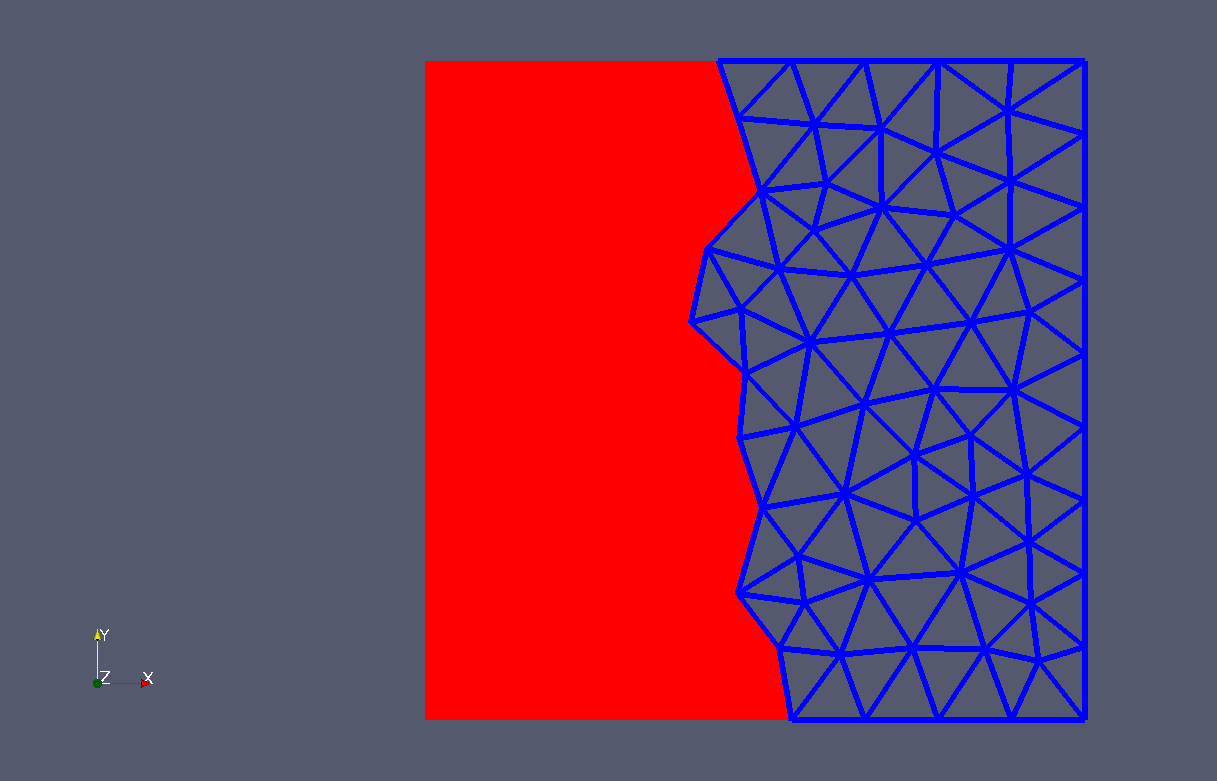
\includegraphics[width=.7\linewidth]{mymeshpartition}
  \label{fig:1}
  \caption{Screenshot of Paraview (3.2.1) of a 2D mesh partitioned and distributed on two processors}
\end{figure}


\subsection{Iterating over the entities of a mesh}

\life mesh data structures provides powerful iterators that allows to
walk though the mesh in various ways: iterate over element, faces ,
points, marked\footnote{associated to an integer flag denoting a
  region, material, processor} elements, marked faces, ...



\section{Function Spaces}
\label{sec:function-spaces}

\subsection{Defining function spaces and functions}

\begin{itemize}
\item basis function
\item function spaces
\item element of a function space
\end{itemize}

\subsection{Using functions spaces and functions}

\begin{itemize}
\item interpolating
\item nodal projection
\item saving
\end{itemize}


\section{Linear Algebra}
\label{sec:linear-algebra}


\life supports three different linear algebra environments that we
shall call \emph{backends}.
\begin{itemize}
\item Gmm\footnote{}
\item Petsc\footnote{}
\item Trilinos\footnote{}
\end{itemize}


\subsection{Choosing a linear algebra backend}
\label{sec:choos-line-algebra}

\index{Class!Backend}\index{boost!shared\_ptr}
To select a backend in order to solve a linear system, we instantiate
the \lstinline!Backend! class associated.

\begin{lstlisting}
#include <life/lifealg/backend.hpp>
boost::shared_ptr<Backend<double> > backend =
     Backend<double>::build( BACKEND_PETSC );
\end{lstlisting}

The backend provides an interface to solve
\begin{equation}
  \label{eq:8}
  A x = b
\end{equation}
\noindent
where $A$ is a $n \times n $ sparse matrix and $x,b$ vectors of size $n$.
The backend defines the \cpp types for  each of these, e.g.
\begin{lstlisting}
Backend<double>::sparse_matrix_type A;
Backend<double>::vector_type x,b;
\end{lstlisting}
\noindent
In practice, we use the \lstinline!boost::shared_ptr<>! shared pointer
to ensure that we won't get memory leaks. The backends provide a
corresponding \lstinline!typedef!


\begin{lstlisting}
Backend<double>::sparse_matrix_ptrtype A( backend->newMatrix( Xh, Yh ) );
Backend<double>::vector_ptrtype x( backend->newVector( Yh ) );
Backend<double>::vector_ptrtype b( backend->newVector( Xh ) );
\end{lstlisting}
\noindent
where $X_h$ and $Y_h$ are function spaces providing the number of
degrees of freedom that will define the size of the matrix and vectors
thanks to the helpers functions \lstinline!Backend::newMatrix()! and
\lstinline!Backend::newVector!. In a parallel setting, the
local/global processor mapping would be passed down by the function
spaces.

\subsection{Defining and using matrices and vectors}
\label{sec:defin-using-matr}

\subsection{Solving}
\label{sec:solving}


\section{Variational Formulation}
\label{sec:vari-form}

\index{formulation!variational}
\begin{itemize}
\item keywords
\item principles
\end{itemize}

\subsection{Computing integrals}
\label{sec:computing-integrals}

\index{integrals}
\marginpar{\lstinline!myintegrals.cpp!}
We would like to compute some integrals on a domain of $\Omega=[0,1]^d\ \subset\ \mathbb{R}^d$
and parts of the domain, i.e. subregions and (parts of) boundary.

Once we have defined the computational mesh, we would like to compute
the area of the domain. We form the integral $\int_\Omega 1$, the code
reads as follows

\lstinputlisting[linerange=marker1-endmarker1]{myintegrals.cpp}

\lstinline!elements(mesh)! returns a pair of iterators over the
elements owned by the current processor, \lstinline!im! is an instance
of the \lstinline!im_type! which provides a quadrature method to
integrate exactly polynomials up to degree 2. In our case integrating
constant(degree 0) would have sufficed, but we will reuse
\lstinline!im! later. Now that we have computed the integral of 1 over
the region of $\Omega$ current processor (ie the area of the domain
owned by the processor), we want to compute the area of $\Omega$. To
do that we collect the integrals on all processors using a
\lstinline!reduce! MPI operation and sum all contributions. We have
used here the Boost.MPI library that provides an extremely powerful
\cpp wrapper around the MPI library. The code reads

\lstinputlisting[linerange=marker2-endmarker2]{myintegrals.cpp}

\noindent
Finally, we print to the log file the result of the local and global
integral calculation. Another calculation is for example to compute
the perimeter of the domain

\lstinputlisting[linerange=marker3-endmarker3]{myintegrals.cpp}

\noindent
the main difference with the domain area computation resides in the
elements with are iterating on: here we are iterating on the boundary
faces of the domain to compute the integral using
\lstinline!boundaryfaces(mesh)! to provide the pairs of iterators.


Now say that we want to compute
\begin{equation}
  \label{eq:5}
  \int_\Omega x^2 + y^2 dx dy.
\end{equation}
The Finite Element Embedded Language (FEEL++) language provides the
keyword \lstinline!Px()! and \lstinline!Py()! to denote the $x$ and
$y$ coordinates like in equation~(\ref{eq:5}).  The code reads then


\lstinputlisting[linerange=marker4-endmarker4]{myintegrals.cpp}

Note that in this case, we really require the use of a quadrature that
integrates exactly order 2 polynomials.

Let's run now the tutrial example \lstinline!myintegrals!. The results are stored
in the log file under \lstinline!~/life/myintegrals/!.

\begin{lstlisting}{language=sh}
> cat ~/life/myintegrals/Simplex_2_1/h_0.5/myintegrals-1.0
myintegrals-1.0 is opened for debug
[Area 0] int_Omega = 1[ 1 ]
[Area 0] int_Omega = 4[ 4 ]
[Area 0] int_Omega = 0.666667[ 0.666667 ]
\end{lstlisting}

We remark that the results are exact. Integrating higher order
polynomials ($\geq 3$) or non-polynomial function would typically
require higher order quadrature to get accurate results. To do that
increase \lstinline!imOrder! in the example and try integrating
$f(x,y)=x^3 + x y^2$.


In order to see what happens in parallel, use \lstinline!mpirun! to
launch \lstinline!myintegrals! on several processors, for example

\begin{lstlisting}{language=sh}
> mpirun -np 4 myintegrals --hsize=0.1
> cat ~/life/myintegrals/Simplex_2_1/h_0.1/myintegrals-4.0
myintegrals-4.0 is opened for debug
[Area 0] int_Omega = 1[ 0.253348 ]
[Area 0] int_Omega = 4[ 1.44444 ]
[Area 0] int_Omega = 0.666667[ 0.0701812 ]
> cat ~/life/myintegrals/Simplex_2_1/h_0.1/myintegrals-4.1
myintegrals-4.1 is opened for debug
[Area 0] int_Omega = 1[ 0.288919 ]
[Area 0] int_Omega = 4[ 0.444444 ]
[Area 0] int_Omega = 0.666667[ 0.186251 ]
> cat ~/life/myintegrals/Simplex_2_1/h_0.1/myintegrals-4.2
myintegrals-4.2 is opened for debug
[Area 0] int_Omega = 1[ 0.183219 ]
[Area 0] int_Omega = 4[ 1.11111 ]
[Area 0] int_Omega = 0.666667[ 0.105008 ]
> cat ~/life/myintegrals/Simplex_2_1/h_0.1/myintegrals-4.3
myintegrals-4.3 is opened for debug
[Area 0] int_Omega = 1[ 0.274514 ]
[Area 0] int_Omega = 4[ 1 ]
[Area 0] int_Omega = 0.666667[ 0.305227 ]
\end{lstlisting}

\subsection{Standard formulation: the Laplacian case}
\label{sec:defin-bilin-forms}
\index{laplacian}
\subsubsection{Mathematical formulation}
\label{sec:math-form-3}
\index{laplacian!formulation!mathematical}
\marginpar{\lstinline!laplacian.cpp!}
In this example, we would like to solve for the following problem in 2D
\begin{problem}
\label{prob:1}
 find $u$ such that
\begin{equation}
  \label{eq:1}
  -\Delta u = f\ \text{in}\ \Omega = [-1;1]^2
\end{equation}
with
\begin{equation}
  \label{eq:2}
  f= 2 \pi^2  g
\end{equation}
and $g$ is the exact solution
\begin{equation}
  \label{eq:3}
  g=\sin(\pi x) \cos(\pi y)
\end{equation}
The following boundary conditions apply
\begin{equation}
  \label{eq:4}
  u=g_{|x=\pm 1}, \quad \frac{\partial u}{\partial n} = 0_{|y=\pm 1}
\end{equation}
\end{problem}

We propose here two possible variational formulations. The first one,
handles the Dirichlet boundary conditions strongly, that is to say the
condition is \emph{incorporated} into the function space definitions.
The second one handles the Dirichlet condition \emph{weakly} and hence
we have a uniform treatment for all types of boundary conditions.



\paragraph{Strong Dirichlet conditions}
\label{sec:strong-dirichl-cond}

\noindent
The variational formulation reads as follows, we introduce the spaces
\begin{equation}
  \label{eq:11}
  \mathcal{X} = \Big\{ v \in H_1(\Omega) \text{ such that } v=g_{|x=-1,x=1} \Big\}
\end{equation}
and
\begin{equation}
  \label{eq:12}
  \mathcal{V} = \Big\{ v \in H_1(\Omega) \text{ such that } v=0_{|x=-1,x=1} \Big\}
\end{equation}
We multiply (\ref{eq:1}) by $v \in \mathcal{V}$ then integrate over $\Omega$ and obtain
\begin{equation}
  \label{eq:13}
  \int_\Omega -\Delta u v = \int_\Omega f v
\end{equation}
We integrate by parts and reformulate the problem as follows:
\begin{problem}
we look
for $u \in \mathcal{X}$ such that for all $v \in \mathcal{V}$
\begin{equation}
  \label{eq:14}
  \int_\Omega \nabla u \cdot \nabla v  = \int_\Omega f v
\end{equation}

\end{problem}
In the present space setting~(\ref{eq:12}) and boundary
conditions~(\ref{eq:4}), we have the boundary term from the integration by
parts which is dropped being equal to 0
\begin{equation}
  \label{eq:15}
  \int_{\partial \Omega} \frac{\partial u}{\partial n} v = 0,
\end{equation}
recalling that
\begin{equation}
  \label{eq:21}
  \frac{\partial u}{\partial n} \stackrel{\text{def}}{=} \nabla u \cdot n
\end{equation}
where $n$ is the outward normal to $\partial \Omega$ by convention.We
now discretize the problem, we create a mesh out of $\Omega$, we have
\begin{equation}
  \label{eq:10}
  \Omega = \cup_{e=1}^\nel \Omega^e
\end{equation}
where $\Omega^e$ can be segments, triangles or tetrahedra depending on
$d$ and we have $\nel$ of them. We introduce the finite dimensional
spaces of continuous piecewise polynomial of degree $N$ functions
\begin{equation}
  \label{eq:17}
  X_h = \Big\{ v_h  \in C^0(\Omega),\ {v_h}_{|\Omega^e} \in \mathbb{P}_N( \Omega^e ),\   v_h=g_{|x=-1,x=1}\Big\}
\end{equation}
and
\begin{equation}
  \label{eq:18}
  V_h = \Big\{ v_h \in C^0(\Omega),\ {v_h}_{|\Omega^e} \in \mathbb{P}_N( \Omega^e ),\   v_h=0_{|x=-1,x=1}\Big\}
\end{equation}
which are out trial and test function spaces respectively.  We now
have the problem we seek to solve which reads in our continuous
Galerkin framework
\begin{problem}
  \label{prob:2}
  we look for $u_h \in X_h \subset \mathcal{X}$ such that for all $v
  \in V_h \subset \mathcal{V}$
  \begin{equation}
    \label{eq:20}
    \int_\Omega \nabla u_h \cdot \nabla v_h  = \int_\Omega f v_h
  \end{equation}
\end{problem}

\paragraph{Weak Dirichlet conditions}
\label{sec:weak-dirichl-cond}

There is an alternative formulation which allows to treat weakly
Dirichlet(Essential) boundary conditions similarly to Neumann(Natural)
and Robin conditions. Following a similar development as in the previous section, the problem reads
\begin{problem}
  \label{prob:3}
  we look for $u \in X_h \subset H_1(\Omega)$ such that for all $v \in
  X_h$
\begin{equation}
  \label{eq:16}
  \int_\Omega \nabla u \cdot \nabla v +
  \int_{|x=-1,x=1} -\frac{\partial u}{\partial n} v - u \frac{\partial v}{\partial n} + \frac{\mu}{h} u v
  =
  \int_\Omega f v +
  \int_{|x=-1,x=1}  - g \frac{\partial v}{\partial n} + \frac{\mu}{h} g v
\end{equation}
where
\begin{equation}
  \label{eq:19}
  X_h = \Big\{ v_h \in C^0(\Omega),\ {v_h}_{|\Omega^e} \in \mathbb{P}_N( \Omega^e ) \Big\}
\end{equation}
\end{problem}
In (\ref{eq:16}), $g$ is defined by (\ref{eq:3}). $\mu$ serves as a penalisation
parameter which should be $> 0$, e.g. between 2 and 10, and $h$ is the
size of the face. The inconvenient of this formulation is the
introduction of the parameter $\mu$, but the advantage is the
\emph{weak} treatment of the Dirichlet condition.

\subsubsection{Life formulation}
\label{sec:life-formulation-1}

\index{laplacian!formulation!life}
First we define the $f$ and $g$. To do that we use the
\lstinline!AUTO! keyword and associate to \lstinline!f! and
\lstinline!g! their expressions

\lstinputlisting[linerange=marker1-endmarker1]{laplacian.cpp}

\noindent where \lstinline!M_PI! is defined in the header
\lstinline!cmath!.  Using \lstinline!AUTO! allows to defined
\lstinline!f!  and \lstinline!g! --- which are moderately complex
object --- without having to know the actual type. \lstinline!AUTO!
determines automatically the type of the expression using the
\lstinline!__typeof__! keyword internally.

Then we form the right hand side by defining a linear form whose
algebraic representation will be stored in a
\lstinline!vector_ptrtype! which is provided by the chosen linear
algebra backend. The linear form is equated with an integral
expression defining our right hand side.

\lstinputlisting[linerange=marker2-endmarker2]{laplacian.cpp}

\noindent \lstinline!form1! generates an instance of the object
representing linear forms, that is to say it mimics the mathematical
object $\ell$ such that
\begin{equation}
  \label{eq:9}
  \begin{array}{rccl}
    \ell: & X_h & \mapsto & \mathbb{R}\\
    & v_h & \rightarrow &\ell(v_h)=\int_\Omega f v
  \end{array}
\end{equation}
which is represented algebraically in the code by the vector
\lstinline!F! using the argument \lstinline!_vector!. The last
argument \lstinline!_init!, if set to \lstinline!true!\footnote{It is
  set to \lstinline!false! by default.}, will zero-out the entries of
the vector \lstinline!F!.


We now turn to the left hand side and define the bilinear form using
the \lstinline!form2! helper function which is passed \textit{(i)} the
trial function space using the \lstinline!_trial! option,
\textit{(ii)} the test function space using the \lstinline!_test!
option, \textit{(iii)} the algebraic representation using
\lstinline!_matrix!, i.e. a sparse matrix whose type is derived from
one of the linear algebra backends and \textit{(iv)} whether the
associated matrix should initialized using
\lstinline!_init!.


\lstinputlisting[linerange=marker3-endmarker3]{laplacian.cpp}


Finally, we deal with the boundary condition, we implement both
formulation described in appendix~\ref{sec:vari-form-1}. For a
\emph{strong} treatment of the Dirichlet condition, we use the
\lstinline!on()! keyword of FEEL++ as follows

\lstinputlisting[linerange=marker5-endmarker5]{laplacian.cpp}

Notice that we add, using \lstinline!+=!, the Dirichlet contribution
for the bilinear form. The first argument is the set of boundary faces
to apply the condition: in gmsh the points satisfying $x=\pm 1$ are
marked using the flags $1$ and $3$ ($x=-1$ and $x=1$ respectively.)

To implement the weak Dirichlet boundary condition, we add the
following contributions to the left and right hand side:

\lstinputlisting[linerange=marker41-endmarker41]{laplacian.cpp}
\lstinputlisting[linerange=marker4-endmarker4]{laplacian.cpp}

Note that we use the command line option \lstinline!--weakdir! set to
1 by default to decide between weak/strong Dirichlet handling.  Apart
the uniform treatment of boundary conditions, the weak Dirichlet
formulation has the advantage to work also in a parallel environment.

Next we solve the linear system
\begin{equation}
  \label{eq:6}
  D u = F
\end{equation}

where the \lstinline!solve! function is implemented as follows

\lstinputlisting[linerange=marker6-endmarker6]{laplacian.cpp}

Finally we check for the $L_2$ error in our approximation by computing
\begin{equation}
  \label{eq:7}
  \|u-u_h\|_{L_2}\ =\ \sqrt{\int_\Omega (u-u_h)^2} = \sqrt{\int_\Omega (g-u_h)^2}
\end{equation}
where $u$ is the exact solution and is equal to $g$ and $u_h$ is the
numerical solution of the problem~(\ref{eq:1}) and the components of
$u_h$ in the $P_2$ Lagrange basis are given by solving (\ref{eq:6}).

The code reads

\lstinputlisting[linerange=marker7-endmarker7]{laplacian.cpp}


You can now verify that the $L_2$ error norm behaves like $h^{-(N+1)}$
where $h$ is the mesh size and $N$ the polynomial order. The $H_1$
error norm would be checked similarly in $h^{-N}$. The
figure~\ref{fig:2} displays the results using Paraview.

\begin{figure}[htbp]
  \centering
  \subfigure[Colored with $u$]{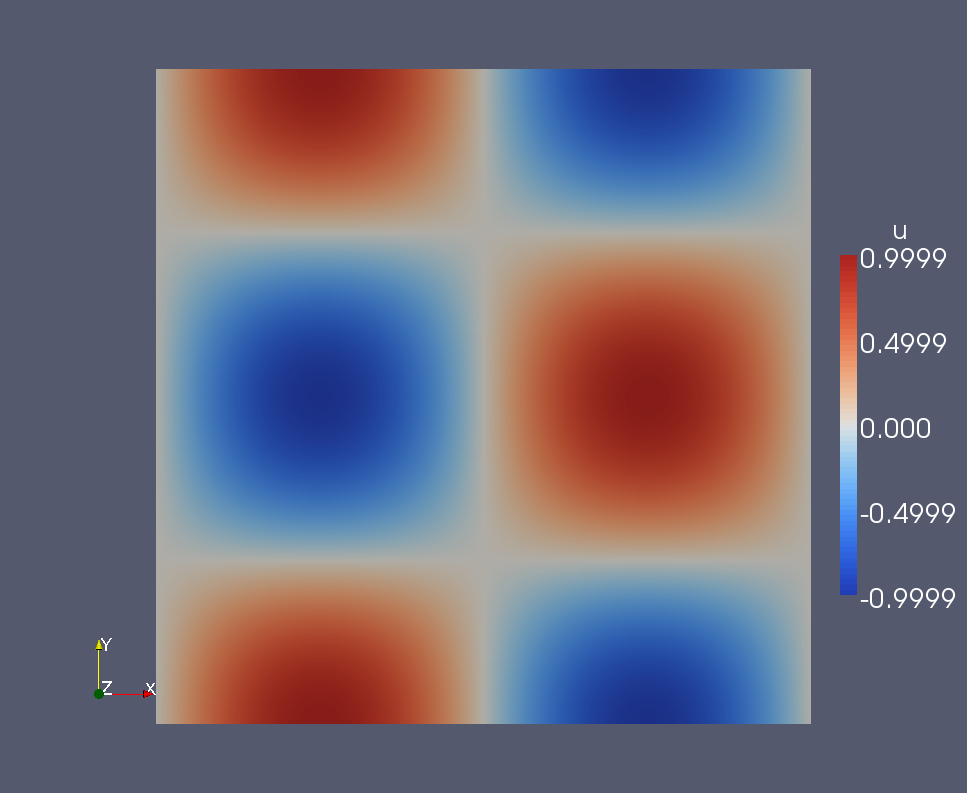
\includegraphics[width=.43\linewidth]{laplacian.png}}
  \subfigure[Elevation]{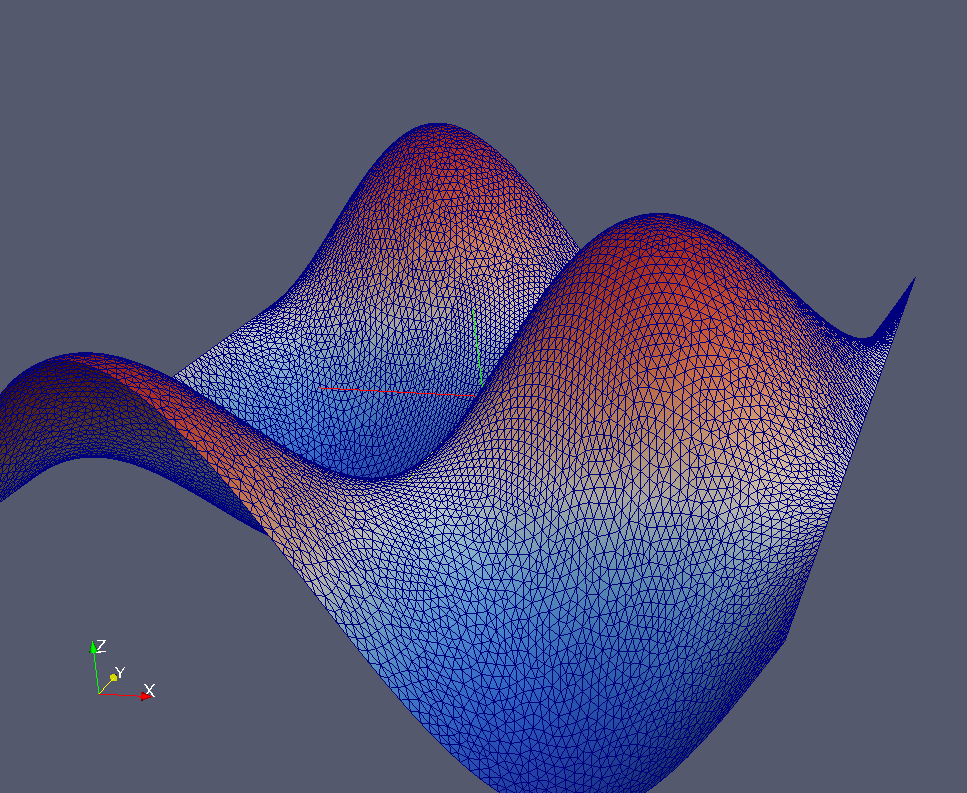
\includegraphics[width=.43\linewidth]{laplacian_warp.png}}
  \caption{Solution of problem~\ref{prob:3}}
  \label{fig:2}
\end{figure}

\subsection{Mixed formulation: the Stokes case}
\label{sec:mixed-form-stok}
\index{Stokes}
\subsubsection{Mathematical formulation}
\label{sec:math-form}

\index{Stokes!formulation!mathematical}
\marginpar{\lstinline!stokes.cpp!}  We are now interested in solving
the Stokes equations, we would like to solve for the following problem
in 2D
\begin{problem}
\label{prob:4}
 find $(\mathbf{u},p)$ such that
\begin{equation}
  \label{eq:22}
  - \mu \Delta \mathbf{u} +\nabla p = \mathbf{f}\quad \text{and}\quad \nabla \cdot \mathbf{u} = 0,\quad \text{in}\ \Omega = [-1;1]^2
\end{equation}
with
\begin{equation}
  \label{eq:24}
  \mathbf{f} = \mathbf{0}
\end{equation}
where $\mu$ being the viscosity. The following boundary conditions apply
\begin{equation}
  \label{eq:23}
  \mathbf{u}=\mathbf{1}_{|y=1}, \quad \mathbf{u}=\mathbf{0}_{|\partial \Omega \backslash \{(x,y) \in \Omega | y=1\}}
\end{equation}
\end{problem}

In problem (\ref{prob:2}), $p$ is known up to a constant $c$,
\emph{i.e.} if $p$ is a solution then $p+c$ is also solution. To
ensure uniqueness we impose the constraint that $p$ should have
zero-mean, \emph{i.e.}
\begin{equation}
  \label{eq:26}
  \int_\Omega p = 0
\end{equation}

The problem~\ref{prob:4} now reads
\begin{problem}
  \label{prob:5}
 find $(\mathbf{u},p,\lambda)$ such that
\begin{equation}
  \label{eq:34}
  - \mu \Delta \mathbf{u} +\nabla p = \mathbf{f}\quad, \quad \nabla \cdot \mathbf{u} + \lambda = 0, \quad \text{and}\quad \int_\Omega p = 0,\quad \text{in}\ \Omega = [-1;1]^2
\end{equation}
with
\begin{equation}
  \label{eq:35}
  \mathbf{f} = \mathbf{0}
\end{equation}
where $\mu$ being the viscosity. The following boundary conditions apply
\begin{equation}
  \label{eq:36}
  \mathbf{u}=\mathbf{1}_{|y=1}, \quad \mathbf{u}=\mathbf{0}_{|\partial \Omega \backslash \{(x,y) \in \Omega | y=1\}}
\end{equation}
\end{problem}

The functional framework is as follows, we look for $\mathbf{u}$ is
$H^1_0(\Omega)$ and $p$ in $L^2_0(\Omega)$. We shall not seek $p$ in
$L^2_0(\Omega)$ but rather in $L^2(\Omega)$ and use Lagrange
multipliers which live are the constants whose space we denote
$\mathbb{P}_0(\Omega)$, to enforce~(\ref{eq:26}).

Denote $\mathcal{X} = H^1_0(\Omega)\times
L^2(\Omega)\times\mathbb{P}_0(\Omega)$, the variational formulation
reads we look for $(\mathbf{u}, p, \lambda) \in \mathcal{X}$ for all
$(\mathbf{v},q,\nu) \in \mathcal{X}$
\begin{equation}
  \label{eq:25}
  \int_\Omega \mu \nabla \mathbf{u} : \nabla \mathbf{v} + \nabla \cdot \mathbf{v} p + \nabla \cdot \mathbf{u}\ q + q \lambda + p \nu  \ = \ \int_\Omega \mathbf{f} \cdot \mathbf{v}
\end{equation}

We build a triangulation $\Omega_h$ of $\Omega$, we choose compatible
(piecewise polynomial) discretisation spaces $X_h$ and $M_h$,
\emph{e.g.} the Taylor Hood element ($\mathbb{P}_N/\mathbb{P}_{N-1}$)
and we denote $\mathcal{X}_h=X_h\times M_h \times
\mathbb{P}_0(\Omega)$.  The discrete problem now reads, we look for
$(\mathbf{u}_h,p_h,\lambda_h) \in \mathcal{X}_h$ such that for all
$(\mathbf{v}_h,q_h,\nu_h) \in \mathcal{X}_h$
\begin{equation}
  \label{eq:27}
  \int_{\Omega_h} \mu \nabla \mathbf{u}_h \cdot \nabla \mathbf{v}_h + \nabla \cdot \mathbf{v}_h \ p_h + \nabla \cdot \mathbf{u}_h\ q_h + p_h \nu_h + q_h \lambda_h   = \ \int_{\Omega_h} \mathbf{f} \cdot \mathbf{v}_h
\end{equation}

The formulation~(\ref{eq:27}) leads to a linear system of the form
\begin{equation}
  \label{eq:28}
  \underbrace{\begin{pmatrix}
    A & B & 0\\
    B^T & 0 & C\\
    0 & C^T & 0
  \end{pmatrix}}_{\mathcal{A}}
\underbrace{
  \begin{pmatrix}
    \mathbf{u}_h\\
    p_h\\
    \lambda_h
  \end{pmatrix}}_{\mathcal{U}} =
\underbrace{\begin{pmatrix}
    F\\
    0\\
    0
  \end{pmatrix}}_{\mathcal{F}}
\end{equation}

where $A$ corresponds to the $(\mathbf{u},\mathbf{v})$ block, $B$ to
the $(\mathbf{u},q)$ block and $C$ to the $(p,\nu)$
block. $\mathcal{A}$ is a symetric positive definite matrix and thus
the system $\mathcal{A} \mathcal{U} = \mathcal{F}$ enjoys a unique
solution.

\subsubsection{Life formulation}
\label{sec:life-formulation}

\index{Stokes!formulation!life}
Regarding the implementation of the Stokes problem~\ref{prob:4}, we
can start from the laplacian case, from
section~\ref{sec:defin-bilin-forms}. The implementation we choose to
display here defines and builds $\mathcal{X}_h$, $\mathcal{A}$,
$\mathcal{U}$ and $\mathcal{F}$.

We start by defining and building $\mathcal{X}_h$: first we define the
basis functions that will span each subspaces $X_h$, $M_h$ and
$\mathbb{P}_0(\Omega)$.

\lstinputlisting[linerange=marker1-endmarker1]{stokes.cpp}

note that on the \lstinline!typedef! we build a (MPL) vector of them. Now we are
ready to define the functionspace $\mathcal{X}_h$, much like in the
Laplacian case:

\lstinputlisting[linerange=marker2-endmarker2]{stokes.cpp}

Next we define a few types which are associated with $\mathcal{U}$,
$u$, $p$ and $\lambda$ respectively.

\lstinputlisting[linerange=marker3-endmarker3]{stokes.cpp}

Using these types we can instantiate elements of $\mathcal{X}_h$,
$X_h$, $M_h$ and $\mathbb{P}_0(\Omega_h)$ respectively:

\lstinputlisting[linerange=marker4-endmarker4]{stokes.cpp}

They will serve in the definition of the variational formulation. We
can now start assemble the various terms of the variational
formulation~(\ref{eq:27}). First we define some viscous stress tensor,
%$\tau(\mathbf{u}) = \frac{1}{2}(\nabla \mathbf{u} + \nabla \mathbf{u}^T)$,
$\tau(\mathbf{u}) = \nabla \mathbf{u}$,
associated with the trial and test functions
respectively

\lstinputlisting[linerange=marker5-endmarker5]{stokes.cpp}

Then we define the total stress tensor times the normal,
$\bar{\sigma}(\mathbf{u},p) \mathbf{n} = -p \mathbf{n} + 2 \mu \tau(\mathbf{u})
\mathbf{n}$ where $\mathbf{n}$ is the normal and $\bar{\sigma}(\mathbf{u},p) =
-p \mathbb{I} + 2 \mu \tau(\mathbf{u})$:

\lstinputlisting[linerange=marker6-endmarker6]{stokes.cpp}


We then form the matrix $\mathcal{A}$ starting with block $A$,  block $B$
block $C$ and finally the boundary conditions.


\lstinputlisting[linerange=marker7-endmarker7]{stokes.cpp}

The figure~\ref{fig:2} displays $p$ and $\mathbf{u}$ which are available in
\begin{unixcom}
  ls ~/life/doc/tutorial/stokes/Simplex_2_1_2/P2/h_0.05
\end{unixcom}

\begin{figure}[htbp]
  \centering
  \subfigure[Colored with $p$, $h=0.05$]{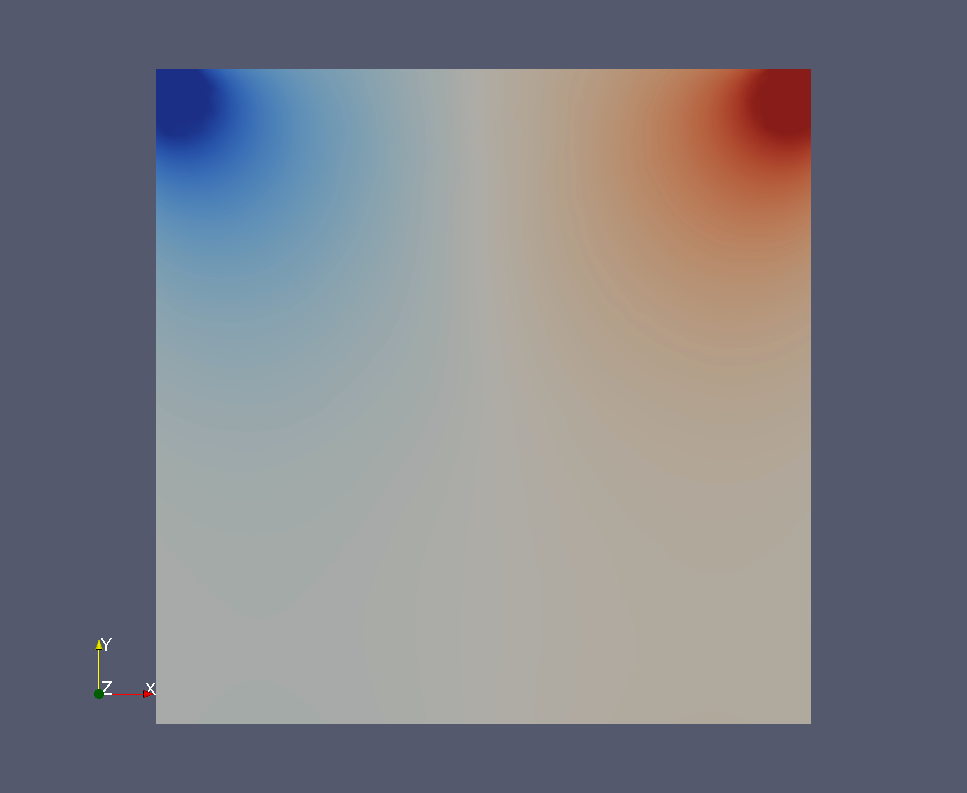
\includegraphics[width=.43\linewidth]{stokes-p.png}}
  \subfigure[Colored with $\|\mathbf{u}\|$ and the arrows associated to $\mathbf{u}$ colored with $p$]{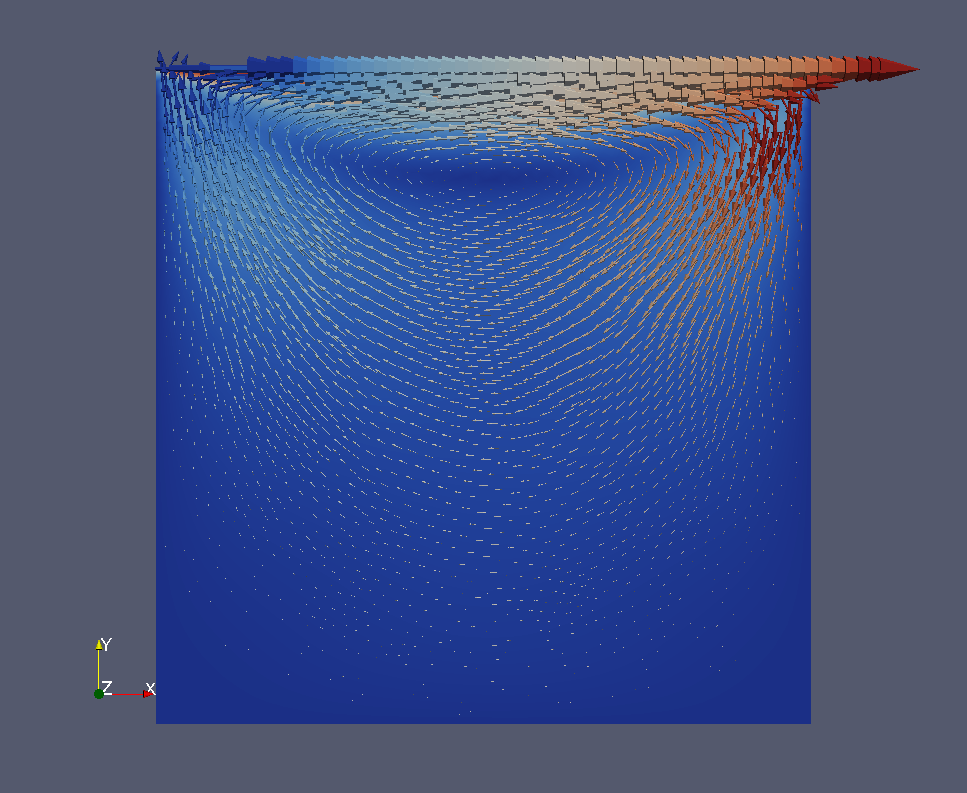
\includegraphics[width=.43\linewidth]{stokes-u.png}}
  \caption{Solution of problem~\ref{prob:4}}
  \label{fig:2}
\end{figure}


\chapter{Examples}
\label{cha:examples}

\section{Solving nonlinear equations}
\label{sec:nonlinear-equations}

\life allows to solve nonlinear equations thanks to its interface to
the interface to the PETSc nonlinear solver library. It requires the
implementation of two extra functions in your application that will
update the jacobian matrix associated to the tangent problem and the
residual.

Consider that you have an application class \lstinline!MyApp! with a
backend as data member
\begin{lstlisting}{gobble=2}
#include <life/lifecore/life.hpp>
#include <life/lifecore/application.hpp>
#include <life/lifealg/backend.hpp>
namespace Life {

class MyApp : public Application
{
  public:

  typedef Backend<double> backend_type;
  typedef boost::shared_ptr<backend_type> backend_ptrtype;

  MyApp( int argc, char** argv,
  AboutData const& ad, po::options_description const& od )
  :
  // init the parent class
  Application( argc, argv, ad, od ),
  // init the backend
  M_backend( backend_type::build( this->vm() ) ),
  {
    // define the callback functions (works only for the PETSc backend)
    M_backend->nlSolver()->residual =
      boost::bind( &self_type::updateResidual, boost::ref( *this ), _1, _2 );
    M_backend->nlSolver()->jacobian =
      boost::bind( &self_type::updateJacobian, boost::ref( *this ), _1, _2 );

  }
  void updateResidual( const vector_ptrtype& X, vector_ptrtype& R )
  {
    // update the matrix J (Jacobian matrix) associated
    // with the tangent problem
  }
  void updateJacobian( const vector_ptrtype& X, sparse_matrix_ptrtype& J)
  {
    // update the vector R associated with the residual
  }
  void run()
  {

    //define space
    Xh...
    element_type u(Xh);
    // initial guess is 0
    u = project( M_Xh, elements(mesh), constant(0.) );
    vector_ptrtype U( M_backend->newVector( u.functionSpace() ) );
    *U = u;

    // define R and J
    vector_ptrtype R( M_backend->newVector( u.functionSpace() ) );
    sparse_matrix_ptrtype J;

    // update R
    updateJacobian( U, R );
    // update J
    updateResidual( U, J );

    // solve using non linear methods (newton)
    // tolerance : 1e-10
    // max number of iterations : 10
    M_backend->nlSolve( J, U, R, 1e-10, 10 );

    // the soluution was stored in U
    u = *U;
  }
  private:

  backend_ptrtype M_backend;
};
} // namespace Life
\end{lstlisting}

The function \lstinline!updateJacobian! and \lstinline!updateResidual!
implement the assmebly of the matrix $J$ (jacobian matrix) and the
vector $R$ (residual vector) respectively.

\subsection{A first nonlinear problem}
\label{sec:bratu}

As a simple example, let $\Omega$ be a subset of $\mathbb{R}^d, d=1,2,3$,
(\emph{i.e.} $\Omega=[-1,1]^d$) with boundary $\partial
\Omega$. Consider now the following equation and boundary condition
\begin{equation}
  \label{eq:29}
  -\Delta u + u^\lambda = f,\quad u = 0 \text{ on } \partial \Omega.
\end{equation}
where $\lambda \in \mathbb{R_+}$ is a given parameter and $f=1$.


\begin{nota}
  To be described in this section. For now see
  \texttt{doc/tutorial/nonlinearpow.cpp} for an implementation of this
  problem.
\end{nota}

\subsection{Simplified combustion problem: Bratu}
\label{sec:bratu}

As a simple example, let $\Omega$ be a subset of $\mathbb{R}^d, d=1,2,3$,
(\emph{i.e.} $\Omega=[-1,1]^d$) with boundary $\partial
\Omega$. Consider now the following equation and boundary condition
\begin{equation}
  \label{eq:29}
  -\Delta u + \lambda e^u = f,\quad u = 0 \text{ on } \partial \Omega
\end{equation}
where $\lambda$ is a given parameter. Ceci est généralement appellé le
problème de Bratu et apparaît lors de la simplification de modèles de
processus de diffusion non-linéaires par exemple dans le domaine de la
combustion.

\begin{nota}
  To be described in this section. For now see
  \texttt{doc/tutorial/bratu.cpp} for an implementation of this
  problem.
\end{nota}

\newcommand{\Gr}{\ensuremath{\mathrm{Gr}\xspace}}
\renewcommand{\Pr}{\ensuremath{\mathrm{Pr}\xspace}}

\section{Natural convection in a heated tank}

\subsection{Description}
\label{sec:description}

The goal of this project is to simulate the fluid flow under natural
convection: the heated fluid circulates towards the low temperature
under the action of density and gravity differences. Thie phenomenon
is important in the sense it models evacuation of heat, generated by
friction forces for example, with  a cooling fluid.

We shall put in place a simple convection problem in order to study
the phenomenon without having to handle the difficulties of more
complex domaines. We describe then some necessary transformations to
the equations, then we define quantities of interest to be able to
compare the simulations with different parameter values.


\newcommand{\Water}{\text{\textsc{Water}}\xspace}
\newcommand{\Fluid}{\text{\textsc{Fluid}}\xspace}
\tikzstyle{snakearrow} = [decoration={snake,aspect=0.2,segment length=1cm,amplitude=1mm},decorate]

\begin{figure}[htbp]
  \centering
  \begin{tikzpicture}[thick,scale=5]

    %% draw axis
    \draw[->] (-0.6,-0.4) -- (1.1,-0.4) node[right] {$x$} coordinate (x axis);
    \draw[-] (-0.,-0.39) -- (0,-0.41) node[below] {$0$};
    \draw[-] (1.,-0.39) -- (1,-0.41) node[below] {$W$};
    \draw[->] (-0.4,-0.6) -- (-0.4,1.1) node[above] {$y$} coordinate (y axis);
    \draw[-] (-0.39,-0.) -- (-0.41,-0.) node[left] {$0$};
    \draw[-] (-0.39,1.) -- (-0.41,1) node[left] {$1$};

    %% draw top and down walls
    \fill[pattern={north east lines},pattern color=blue] (0,1) rectangle  (1,1.02) ;
    \fill[pattern={north west lines},pattern color=blue] (0,0) rectangle  (1,-0.02) ;

    %% Draw the domain
    \draw[very thick,fill=blue!10!white,draw=blue!50] (0,0) rectangle  (1,1) ;
    \node at (0.1,0.5) {$\Gamma_1$};
    \node at (0.5,0.1) {$\Gamma_2$};
    \node at (0.9,0.5)  {$\Gamma_3$};
    \node at (0.8,0.9)  {$\Gamma_4$};
    \node (omega) at (0.5,0.3)  {$\Omega (\Fluid)$};
    % \draw[->,snakearrow] (omega) -- (0.5,0.5);
    \draw[<->] (0,-0.1) -- (1,-0.1) node [below,midway] {$W$};
    \draw[-] (0.5,1.) -- (0.5,0.5) node[left,midway] {$\Gamma_f$};
    \draw[-,ultra thick,color=blue] (0,0) -- (0,1) node [left,midway] {$T_0$};
    \draw[-,ultra thick,color=red] (1,0) -- (1,1)  {};


    \foreach \y in {0.1,0.3,0.5,0.7,0.9} {
      %%\draw[->] (\x, -1.5) -- (\x,\pgfmathqparse{-0.7*\x*\x+0.7*8*\x-12} \pgfmathresult);
      %%\pgfmathsetmacro{\pgf@x}{\x}
      %%\pgfmathparse{-0.7*\pgf@x*\pgf@x+0.7*8*\pgf@x-0.7*12}
      %%\def\y{\pgfmathresult}
      \def\x{1.3}
      \draw[->] (1.3, \y) -- (1.1,\y);
    }
    \node at (1.6,0.5) {Heat flux};

  \end{tikzpicture}
  \caption{Geometry of the model}
  \label{fig:heatns:1}
\end{figure}

To study the convection, we use a model problem: it consists in a
rectangular tank of height $1$ and width $W$, in which the fluid is
enclosed, see figure~\vref{fig:heatns:1}. We wish to know the fluid velocity
$\mathbf{u}$, the fluid pressure $p$ and fluid temperature $\theta$.

We introduce the adimensionalized Navier-Stokes and heat equations
parametrized by the Grashof and Prandtl numbers. These parameters
allow to describe the various regimes of the fluid flow and heat
transfer in the tank when varying them.

The adimensionalized steady incompressible Navier-Stokes equations reads:
\begin{equation}
  \label{eq:38}
  \begin{split}
    \mathbf{u}\cdot\nabla \mathbf{u} +\nabla p -\frac{1}{\sqrt{\Gr}} \Delta \mathbf{u} &= \theta \mathbf{e}_2\\
    \nabla \cdot \mathbf{u} & = 0\ \text{sur}\ \Omega\\
    \mathbf{u} & = \mathbf{0}\ \text{sur}\ \partial \Omega
  \end{split}
\end{equation}
where $\Gr$ is the Grashof number, $\mathbf{u}$ the adimensionalized
velocity and $p$ adimensionalized pressure and $\theta$ the
adimensionalized temperature. The temperature is in fact the
difference between the temperature in the tank and the temperature
$T_0$ on boundary $\Gamma_1$.

The heat equation reads:
\begin{equation}
  \label{eq:37}
  \begin{split}
    \mathbf{u} \cdot \nabla \theta -\frac{1}{\sqrt{\Gr}\Pr} \Delta \theta &= 0\\
    \theta &= 0\ \text{sur}\ \Gamma_1\\
    \frac{\partial \theta}{\partial n} &= 0\ \text{sur}\ \Gamma_{2,4}\\
    \frac{\partial \theta}{\partial n} &= 1\ \text{sur}\ \Gamma_3
  \end{split}
\end{equation}
where $\Pr$ is the Prandtl number.

% \subsection{Nombre de Grashof}
% \label{sec:nombre-de-grashof}
% Le nombre de Grashof (\Gr) est un nombre sans dimension utilisé en
% mécanique des fluides pour caractériser la convection libre dans un
% fluide. Il correspond au rapport des forces de gravité sur les forces
% visqueuses.

% On le définit de la manière suivante
% \begin{equation}
%   \label{eq:18}
%   \Gr = \frac{g\  \beta\  (T-T_\infty)\  {L_c}^3}{\nu^2}
% \end{equation}
% avec:
% \begin{itemize}
% \item $g$ - constante gravitationnelle
% \item $\beta$ - coefficient de dilatation
% \item $T-T_\infty$ - différence de température
% \item $L_c$ - longueur caractéristique
% \item $\nu$ - viscosité cinématique
% \end{itemize}

% \subsection{Nombre de Prandtl}
% \label{sec:nombre-de-prandtl}

% Le nombre de Prandtl (\Pr) est un nombre sans dimension. Il représente
% le rapport entre la diffusivité de quantité de mouvement $\nu$ (ou
% viscosité cinématique) et la diffusivité thermique.

% On le définit de la manière suivante
% \begin{equation}
%   \label{eq:19}
%   \Pr=\frac {\mu C_p }{\lambda}=\frac {\mu}{\frac {k}{C_p}}=\frac {\frac {\mu}{\rho}}{\frac {k}{\rho C_p}}=\frac {\nu}{\alpha}
% \end{equation}
% avec
% \begin{itemize}
% \item $\nu$ la viscosité cinématique en $m^2\cdot s^{-1}$
% \item $\rho$ la masse volumique en $kg\cdot m^{-3}$
% \item $\alpha$ la diffusivité thermique en $m^2\cdot s^{-1}$
% \item $\mu$ la viscosité dynamique en $N\cdot s\cdot m^{-2}$
% \item $C_p$ la chaleur massique en $J\cdot kg^{-1}\cdot K^{-1}$
% \item $k$ la conductivité thermique $W \cdot m^{-1}\cdot K^{-1}$
% \end{itemize}



\subsection{Influence of parameters}
\label{sec:infl-des-param}


what are the effects of the Grashof and Prandtl numbers ? We remark
that both terms with these parameters appear in front of the $\Delta$
parameter, they thus act on the diffusive terms. If we increase the
Grashof number or the Prandtl number the coefficients multiplying the
diffusive terms decrease, and this the convection, that is to say the
transport of the heat via the fluid, becomes dominant. This leads also
to a more difficult and complex flows to simulate, see
figure~\ref{fig:heatns:2}. The influence of the Grashof and Prandtl
numbers are different but they generate similar difficulties and flow
configurations. Thus we look only here at the influence of the Grashof
number which shall vary in $[1, 1e7]$.

\begin{figure}[htbp]
  \centering
  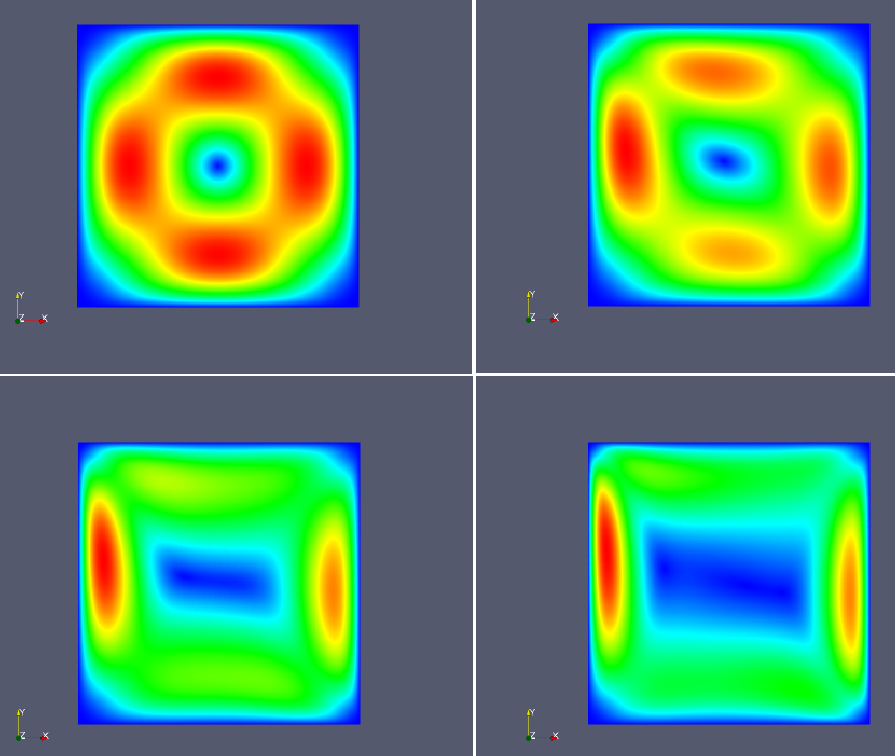
\includegraphics[width=.8\linewidth]{pngs/flow_grashof}
  \caption{Velocity norm with respect to  Grashof, $\Gr=100, 10000,
    100000, 500000$. $h=0.01$ and $\Pr=1$.}
  \label{fig:heatns:2}
\end{figure}

\subsection{Quantities of interest}
\label{sec:quant-du-benchm}

We would like to compare the results of many simulations with respect
to the Grashof defined in the previous section. We introduce two
quantities which will allow us to observe the behavior of the flow and
heat transfer.


\subsubsection{Mean temperature}
\label{sec:mean-temperature}

We consider first the mean temperature on boundary $\Gamma_3$
\begin{equation}
  \label{eq:16}
  T_3 = \int_{\Gamma_3} \theta
\end{equation}

This quantity should decrease with increasing Grashof because the
fluid flows faster and will transport more heat which will cool down
the heated boundary $\Gamma_3$. We observe this behavior on the
figure~\ref{fig:heatns:3}.

\begin{figure}[htbp]
  \centering
  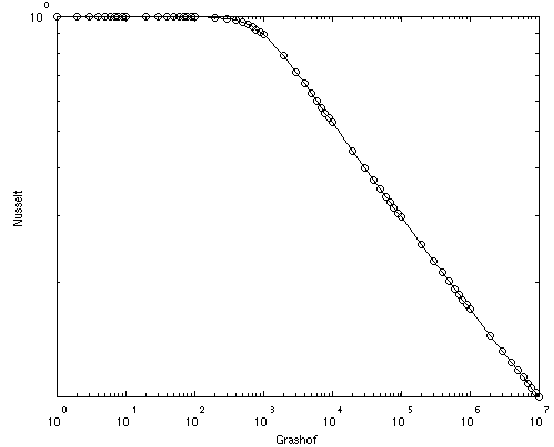
\includegraphics[width=.8\linewidth]{pngs/temp_grashof}
  \caption{Mean temperature with respect to the Grashof number;
    $h=0.02$ with $\mathbb{P}_3$ Lagrange element for the velocity,
    $\mathbb{P}_2$ Lagrange for the pressure and $\mathbb{P}_1$
    Lagrange for the temperature.}
  \label{fig:heatns:3}
\end{figure}

\subsubsection{Flow rate}
\label{sec:flow-rate}

Another quantity of interest is the flow rate through the middle of the
tank. We define a segment $\Gamma_f$ as being the vertical top
semi-segment located at $W/2$ with height $1/2$, see
figure~\ref{fig:heatns:1}. The flow rate, denoted $\mathrm{D}_f$, reads
\begin{equation}
  \label{eq:17}
  \mathrm{D}_f =  \int_{\Gamma_f} \mathbf{u} \cdot \mathbf{e}_1
\end{equation}
where $\mathbf{e}_1=(1,0)$. Note that the flow rate can be negative or
positive depending on the direction in which the fluid flows.

As a function of the Grashof, we shall see a increase in the flow
rate. This is true for small Grashof, but starting at $1e3$ the flow
rate decreases. The fluid is contained in a boundary layer which is
becoming smaller as the Grashof increases.

\begin{figure}[htbp]
  \centering
  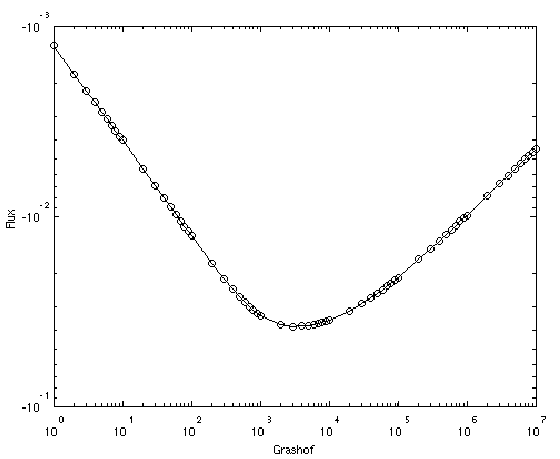
\includegraphics[width=.8\linewidth]{pngs/debit_grashof}
  \caption{Behavior of the flow rate with respect to the Grashof number; $h = 0.02$,
    $\mathbb{P}_3$ for the velocity, $\mathbb{P}_2$ for the pressure and
    $\mathbb{P}_1$ for the temperature.}
  \label{fig:4}
\end{figure}




%%% Local Variables:
%%% coding: utf-8
%%% mode: latex
%%% TeX-PDF-mode: t
%%% TeX-parse-self: t
%%% x-symbol-8bits: nil
%%% TeX-auto-regexp-list: TeX-auto-full-regexp-list
%%% TeX-master: "life-manual"
%%% ispell-local-dictionary: "american"
%%% End:


% The discrete variational formulation reads, we look for $u \in V
% \subset H^1(\Omega)$ such that
% \begin{equation}
%   \label{eq:30}
%   \int_\Omega \nabla u \cdot \nabla v + \lambda e^u v + \int_{\partial \Omega} -\frac{\partial u}{\partial \mathbf{n}} v -\frac{\partial v}{\partial \mathbf{n}} u + \frac{\mu}{h} u v  = 0\quad \forall v \in V
% \end{equation}
% where the last terms integrate on $\partial \Omega$ are associated with the weak treatment of the Dirichlet condition, see~\ref{sec:weak-dirichl-cond}.
% Denote the residual
% \begin{equation}
%   \label{eq:31}
%   \mathcal{F}() v=  \int_\Omega \nabla u \cdot \nabla v + \lambda e^u v + \int_{\partial \Omega} -\frac{\partial u}{\partial \mathbf{n}} v -\frac{\partial v}{\partial \mathbf{n}} u + \frac{\mu}{h} u v
% \end{equation}
% Denote the Jacobian
% \begin{equation}
%   \label{eq:32}
%   \mathcal{J}_z(u,v) = \int_\Omega \lambda e^z u v + \underbrace{\int_\Omega \nabla u \cdot \nabla v + \int_{\partial \Omega} -\frac{\partial u}{\partial \mathbf{n}} v -\frac{\partial v}{\partial \mathbf{n}} u + \frac{\mu}{h} u v}_{\text{linear part, constant over the nonlinear iterations}}
% \end{equation}
% The Nonlinear iterations now reads if $J$ and $F$ are the matrices and
% vectors associated with $\mathcal{J}_z$ and $\mathcal{F}$ respectively: given $u^{0}$
% \begin{equation}
%   \label{eq:33}
%   J_{u^n} u^{n+1} = -F
% \end{equation}



\appendix
\newpage
% \chapter{Compiling the tutorial examples}
% \label{sec:comp-tutor-exampl}


% \section{CMake}

% The build system of the tutorial examples is
% CMake\footnote{\url{http://www.cmake.org}} by Kitware.Here is a excerpt from CMake web site

% CMake is a cross-platform, open-source make system. CMake is used to
% control the software compilation process using simple platform and
% compiler independent configuration files. CMake generates native
% makefiles and workspaces that can be used in the compiler environment
% of your choice. CMake is quite sophisticated: it is possible to
% support complex environments requiring system configuration,
% pre-processor generation, code generation, and template
% instantiation. Please go here to learn more about CMake.

% CMake was developed by Kitware as part of the NLM Insight Segmentation
% and Registration Toolkit project. The ASCI VIEWS project also provided
% support in the context of their parallel computation
% environment. Other sponsors include the Insight, VTK, and VXL open
% source software communities.

% The goals for CMake include the following:

% \begin{itemize}
% \item Develop an open source, cross-platform tool to manage the build process,
% \item Allow the use of native compilers and systems,
% \item Simplify the build process,
% \item Optionally provide a user-interface to manage the build system,
% \item Create an extensible framework,
% \item Grow a self-sustaining community of software users and developers.
% \end{itemize}

% \section{Building the examples}
% \label{sec:building-examples}

% The compilation is fairly simple. First make sure that the
% \lstinline!cmake! and eventually its text based(ncurses) interfaces
% \lstinline!ccmake! are in your \lstinline!PATH! (i.e. you can execute
% them).
% \noindent
% Then create a directory, where you will build and test the examples, e.g.
% \begin{lstlisting}{language=sh}
% mkdir tutorial-build
% cd tutorial-build
% \end{lstlisting}

% \noindent
% Then you configure and generate the \lstinline!Makefile!s using CMake
% \begin{lstlisting}{language=sh}
% cmake <path to tutorial sources>
% \end{lstlisting}
% \noindent
% CMake provides a text based interface using ncurses for configuration,
% you can check it out using the command
% \begin{lstlisting}{language=sh}
% ccmake <path to tutorial sources>
% \end{lstlisting}
% \noindent Follow the instructions at the bottom: press \lstinline!c!
% to configure, then \lstinline!g! to generate the \lstinline!Makefile!s

% \noindent
% You are now ready to compile the examples
% \begin{lstlisting}{language=sh}
% make
% \end{lstlisting}
% If somehow something fails during the build, try using the
% \lstinline!make!  option \lstinline!-k! which allows to continue
% after a failure.


\feelchapter{Feel++ Language Keywords}
            {Feel++ Language Keywords}
            {Christophe Prud'homme}
            {cha:appendix-feel}

One of Life assets is it finite element embedded language
(\feel). The language follows the C++ grammar, and provides keywords
as well as operations between objects which are, mathematically,
tensors of rank 0, 1 or 2.

Some notations
\begin{itemize}
\item $f: \mathbb{R}^n \mapsto \mathbb{R}^{m\times p}$  with $n=1,2,3$, $m=1,2,3$, $p=1,2,3$.
\item $\Omega^e$ current mesh element
\end{itemize}


\begin{longtable}[c]{rllll}
  Keyword & Math object & Description & Rank & $M \times N$\\\hline\hline

  \endhead
  %%
  %% Point
  %%
  \lstinline!P()! & $\overrightarrow{P}$ & current point coordinates $(P_x, P_y, P_z)^T$ & 1 & $d \times 1$ \\

  \lstinline!Px()! & $P_x$ & $x$ coordinate of $\overrightarrow{P}$ & 0 & $1 \times 1$\\

  \lstinline!Py()! & $P_y$ & $y$ coordinate of $\overrightarrow{P}$ & 0 & $1 \times 1$\\
  & &  (value is 0 in 1D) & &\\

  \lstinline!Pz()! & $P_z$ & $z$ coordinate of $\overrightarrow{P}$& 0 & $1 \times 1$\\
  & &  (value is 0 in 1D and 2D)  & &\\\hline\\

  %%
  %% Barycenter
  %%
  \lstinline!C()! & $\overrightarrow{C}$ & element barycenter point coordinates  & 1 & $d \times 1$ \\
  &&$(C_x, C_y, C_z)^T$&&\\

  \lstinline!Cx()! & $C_x$ & $x$ coordinate of $\overrightarrow{C}$ & 0 & $1 \times 1$\\

  \lstinline!Cy()! & $C_y$ & $y$ coordinate of $\overrightarrow{C}$ & 0 & $1 \times 1$\\
  & &  (value is 0 in 1D) & &\\

  \lstinline!Cz()! & $C_z$ & $z$ coordinate of $\overrightarrow{C}$& 0 & $1 \times 1$\\
  & &  (value is 0 in 1D and 2D)  & &\\\hline\\

  %%
  %% normal
  %%

  \lstinline!N()! & $\overrightarrow{N}$ & normal at current point $(N_x,N_y,N_z)^T$ & 1 & $d \times 1$\\

  \lstinline!Nx()! & $N_x$ & $x$ coordinate of $\overrightarrow{N}$ at current point & 0 & $1 \times 1$\\

  \lstinline!Ny()! & $N_y$ & $y$ coordinate of $\overrightarrow{N}$ at current point & 0 & $1 \times 1$\\
  & &  (value is 0 in 1D) & &\\

  \lstinline!Nz()! & $N_z$ & $z$ coordinate of $\overrightarrow{N}$ at current point& 0 & $1 \times 1$\\
  & &  (value is 0 in 1D and 2D)  & &\\\hline\\

  %%
  %% Element id
  %%
  \lstinline!eid()! & $e$ & index of  $\Omega^e$ & 0 & $1 \times 1$\\
  \lstinline!emarker()! & $m(e)$ & marker of  $\Omega^e$ & 0 & $1 \times 1$\\
  \lstinline!h()! & $h^e$ & size of   $\Omega^e$ & 0 & $1 \times 1$\\
  \lstinline!hFace()! & $h^e_{\Gamma}$ & size of face $\Gamma$ of $\Omega^e$ & 0 & $1 \times 1$\\\hline\\

  %%
  %% Mat/vec
  %%
  \lstinline!mat<M,N>(m_11,! &
  $\begin{pmatrix}
    m_{11} & m_{12} & ...\\
    m_{21} & m_{22} & ...\\
    \vdots & &
  \end{pmatrix}$
  & $M\times N$ matrix    & 2 & $M \times N$\\
  \lstinline!m_12,...)!& & entries being expressions   & &\\

  \lstinline!vec<M>(v_1,! &$(v_1, v_2,...)^T$
  & column vector with $M$ rows    & 1 & $M \times 1$\\
  \lstinline!v_2,...)!& & entries being expressions   & &\\

  \lstinline!trace(expr)! &$\mathrm{tr}(f(\overrightarrow{x}))$  & trace of $f(\overrightarrow{x})$   & 0 & $1 \times 1$\\\hline\\


  %%
  %% std math functions
  %%

  \lstinline!abs(expr)! & $|f(\overrightarrow{x})|$ & element wise absolute value of $f$ & $\mathrm{rank}(f(\overrightarrow{x}))$ & $m \times p$\\
  \lstinline!cos(expr)! & $\cos(f(\overrightarrow{x}))$ & element wise cosinus value of $f$ & $\mathrm{rank}(f(\overrightarrow{x}))$ & $m \times p$\\
  \lstinline!sin(expr)! & $\sin(f(\overrightarrow{x}))$ & element wise sinus value of $f$ & $\mathrm{rank}(f(\overrightarrow{x}))$ & $m \times p$\\
  \lstinline!tan(expr)! & $\tan(f(\overrightarrow{x}))$ & element wise tangent value of $f$ & $\mathrm{rank}(f(\overrightarrow{x}))$ & $m \times p$\\
  \lstinline!acos(expr)! & $\acos(f(\overrightarrow{x}))$ & element wise acos value of $f$ & $\mathrm{rank}(f(\overrightarrow{x}))$ & $m \times p$\\
  \lstinline!asin(expr)! & $\asin(f(\overrightarrow{x}))$ & element wise asin value of $f$ & $\mathrm{rank}(f(\overrightarrow{x}))$ & $m \times p$\\
  \lstinline!atan(expr)! & $\atan(f(\overrightarrow{x}))$ & element wise atan value of $f$ & $\mathrm{rank}(f(\overrightarrow{x}))$ & $m \times p$\\
  \lstinline!cosh(expr)! & $\cosh(f(\overrightarrow{x}))$ & element wise cosh value of $f$ & $\mathrm{rank}(f(\overrightarrow{x}))$ & $m \times p$\\
  \lstinline!sinh(expr)! & $\sinh(f(\overrightarrow{x}))$ & element wise sinh value of $f$ & $\mathrm{rank}(f(\overrightarrow{x}))$ & $m \times p$\\
  \lstinline!tanh(expr)! & $\tanh(f(\overrightarrow{x}))$ & element wise tanh value of $f$ & $\mathrm{rank}(f(\overrightarrow{x}))$ & $m \times p$\\
  \lstinline!exp(expr)! & $\exp(f(\overrightarrow{x}))$ & element wise exp value of $f$ & $\mathrm{rank}(f(\overrightarrow{x}))$ & $m \times p$\\
  \lstinline!log(expr)! & $\log(f(\overrightarrow{x}))$ & element wise log value of $f$ & $\mathrm{rank}(f(\overrightarrow{x}))$ & $m \times p$\\
  \lstinline!sqrt(expr)! & $\sqrt{f(\overrightarrow{x})}$ & element wise sqrt value of $f$ & $\mathrm{rank}(f(\overrightarrow{x}))$ & $m \times p$\\
  \lstinline!sign(expr)! & $
  \begin{cases}
    1 & \text{if}\ f(\overrightarrow{x}) \geq 0\\
    -1 & \text{if}\ f(\overrightarrow{x}) < 0
  \end{cases}$ & element wise sign of $f$ & $\mathrm{rank}(f(\overrightarrow{x}))$ & $m \times p$\\
  \lstinline!chi(expr)! & $\chi(f(\overrightarrow{x}))=$ & element wise boolean test of $f$ & $\mathrm{rank}(f(\overrightarrow{x}))$ & $m \times p$\\
  & $\begin{cases}
    0 & \text{if}\ f(\overrightarrow{x}) = 0\\
    1 & \text{if}\ f(\overrightarrow{x}) \neq 0\\
  \end{cases}$ &&&\\\hline\\

  %%
  %% operation
  %%
  \lstinline!id(f)! & $f$ & test function & $\mathrm{rank}(f(\overrightarrow{x}))$ & $m \times p$\\
  \lstinline!idt(f)! & $f$ & trial function & $\mathrm{rank}(f(\overrightarrow{x}))$ & $m \times p$\\
  \lstinline!idv(f)! & $f$ & evaluation function   & $\mathrm{rank}(f(\overrightarrow{x}))$ & $m \times p$\\
  \lstinline!grad(f)! & $\nabla f$ & gradient of test function & $\mathrm{rank}( f(\overrightarrow{x}))+1$ & $p=1,\ m \times n$\footnote{Gradient of matrix value functions is not implemented, hence $p=1$ }\\
  \lstinline!gradt(f)! & $\nabla f$ & gradient of trial function & $\mathrm{rank}(f(\overrightarrow{x}))+1$ & $p=1,\ m \times n$\\
  \lstinline!gradv(f)! & $\nabla f$ & evaluation function gradient    & $\mathrm{rank}(f(\overrightarrow{x}))+1$ & $p=1,\ m \times n$\\

  \lstinline!div(f)! & $\nabla \cdot \overrightarrow{f}$ & divergence of test function & $\mathrm{rank}( f(\overrightarrow{x}))-1$ & $1\times 1$\footnote{Divergence  of matrix value functions is not implemented, hence $p=1$ }\\
  \lstinline!divt(f)! & $\nabla \cdot \overrightarrow{f}$ & divergence of trial function & $\mathrm{rank}( f(\overrightarrow{x}))-1$ & $1\times 1$\\
  \lstinline!divv(f)! & $\nabla \cdot \overrightarrow{f}$ & evaluation of  function divergence  & $\mathrm{rank}( f(\overrightarrow{x}))-1$ & $1\times 1$\\

  \lstinline!curl(f)! & $\nabla \times \overrightarrow{f}$ & curl of test function & 1 & $n=m, n\times 1$\\
  \lstinline!curlt(f)! & $\nabla \times \overrightarrow{f}$ & curl of trial function & 1 & $m=n, n\times 1$\\
  \lstinline!curlv(f)! & $\nabla \times \overrightarrow{f}$ & evaluation of  function curl  & 1 & $m=n, n\times 1$\\

  \lstinline!hess(f)! & $\nabla^2 f$ & hessian of test function & 2 & $m=p=1, n\times n$\\\hline\\

  %%
  %% Two valued operators
  %%
  \lstinline!jump(f)! & $[f]=f_0\overrightarrow{N_0}+f_1\overrightarrow{N_1}$ & jump of test function & 1   & $m=1, n\times 1$\\
  \lstinline!jump(f)! & $[\overrightarrow{f}]=\overrightarrow{f_0}\cdot\overrightarrow{N_0}+\overrightarrow{f_1}\cdot\overrightarrow{N_1}$ & jump of test function & 0   & $m=2, 1\times 1$\\
  \lstinline!jumpt(f)! & $[f]=f_0\overrightarrow{N_0}+f_1\overrightarrow{N_1}$ & jump of trial function & 1   & $m=1, n\times 1$\\
  \lstinline!jumpt(f)! & $[\overrightarrow{f}]=\overrightarrow{f_0}\cdot\overrightarrow{N_0}+\overrightarrow{f_1}\cdot\overrightarrow{N_1}$ & jump of trial function & 0   & $m=2, 1\times 1$\\
  \lstinline!jumpv(f)! & $[f]=f_0\overrightarrow{N_0}+f_1\overrightarrow{N_1}$ & jump of  function evaluation & 1   & $m=1, n\times 1$\\
  \lstinline!jumpv(f)! & $[\overrightarrow{f}]=\overrightarrow{f_0}\cdot\overrightarrow{N_0}+\overrightarrow{f_1}\cdot\overrightarrow{N_1}$ & jump of  function evaluation & 0   & $m=2, 1\times 1$\\
  \lstinline!average(f)! & ${f}=\frac{1}{2}(f_0+f_1)$ & average of test function & $\mathrm{rank}( f(\overrightarrow{x}))$   & $m=n, n\times n$\\
  \lstinline!averaget(f)! & ${f}=\frac{1}{2}(f_0+f_1)$ & average of trial function & $\mathrm{rank}( f(\overrightarrow{x}))$   & $m=n, n\times n$\\
  \lstinline!averagev(f)! & ${f}=\frac{1}{2}(f_0+f_1)$ & average of  function evaluation & $\mathrm{rank}( f(\overrightarrow{x}))$   & $m=n, n\times n$\\

  \lstinline!leftface(f)! & $f_0$ & left  test function & $\mathrm{rank}( f(\overrightarrow{x}))$   & $m=n, n\times n$\\
  \lstinline!leftfacet(f)! & $f_0$ & left  trial function & $\mathrm{rank}( f(\overrightarrow{x}))$   & $m=n, n\times n$\\
  \lstinline!leftfacev(f)! & $f_0$ & left   function evaluation & $\mathrm{rank}( f(\overrightarrow{x}))$   & $m=n, n\times n$\\
  \lstinline!rightface(f)! & $f_1$ & right  test function & $\mathrm{rank}( f(\overrightarrow{x}))$   & $m=n, n\times n$\\

  \lstinline!rightfacet(f)! & $f_1$ & right  trial function & $\mathrm{rank}( f(\overrightarrow{x}))$   & $m=n, n\times n$\\
  \lstinline!rightfacev(f)! & $f_1$ & right   function evaluation & $\mathrm{rank}( f(\overrightarrow{x}))$   & $m=n, n\times n$\\

  \lstinline!maxface(f)! & $\max(f_0,f_1)$ & maximum of right and left & $\mathrm{rank}( f(\overrightarrow{x}))$   & $m\times p$\\
  && test   function&&\\
  \lstinline!maxfacet(f)! & $\max(f_0,f_1)$ & maximum of right and left & $\mathrm{rank}( f(\overrightarrow{x}))$   & $m\times p$\\
  && trial   function&&\\
  \lstinline!maxfacev(f)! & $\max(f_0,f_1)$ & maximum of right and left & $\mathrm{rank}( f(\overrightarrow{x}))$   & $m\times p$\\
  && function evaluation&&\\
  \lstinline!minface(f)! & $\min(f_0,f_1)$ & minimum of right and left & $\mathrm{rank}( f(\overrightarrow{x}))$   & $m\times p$\\
  && test   function&&\\
  \lstinline!minfacet(f)! & $\min(f_0,f_1)$ & minimum of right and left & $\mathrm{rank}( f(\overrightarrow{x}))$   & $m\times p$\\
  && trial   function&&\\
  \lstinline!minfacev(f)! & $\min(f_0,f_1)$ & minimum of right and left & $\mathrm{rank}( f(\overrightarrow{x}))$   & $m\times p$\\
  && function evaluation&&\\
  \hline\\
  %%
  %% Operations
  %%
  \lstinline!-! & $-g$ & element wise unary minus  & & \\
  \lstinline!-! & $!g$ & element wise logical not  & & \\\hline\\

  \lstinline!+! & $f+g$ & tensor sum  & & \\
  \lstinline!-! & $f-g$ & tensor substraction  & & \\
  \lstinline!*! & $f*g$ & tensor product  & & \\
  \lstinline!/! & $f/g$ & tensor division ($g$ scalar field)  & & \\\hline\\

  \lstinline!<! & $f < g$ & element wise less  & & \\
  \lstinline!<=! & $f \leq g$ & element wise less or equal  & & \\
  \lstinline!>! & $f > g$ & element wise greater  & & \\
  \lstinline!>=! & $f \geq g$ & element wise greater or equal  & & \\
  \lstinline!==! & $f = g$ & element wise  equal  & & \\
  \lstinline+!=+ & $f \neq g$ & element wise not equal  & & \\
  \lstinline!&&! & $f\ \text{and}\ g$ & element wise logical and  & & \\
  \lstinline!||! & $f\ \text{or}\ g$ & element wise logical or  & & \\\hline\\


\end{longtable}
%%% Local Variables:
%%% coding: utf-8
%%% mode: latex
%%% TeX-PDF-mode: t
%%% TeX-parse-self: t
%%% x-symbol-8bits: nil
%%% TeX-auto-regexp-list: TeX-auto-full-regexp-list
%%% TeX-master: "feel-manual"
%%% ispell-local-dictionary: "american"
%%% End:


\chapter{GNU Free Documentation License}
\label{sec:gnu-free-docum}

		GNU Free Documentation License
		  Version 1.2, November 2002


 Copyright (C) 2000,2001,2002  Free Software Foundation, Inc.
     51 Franklin St, Fifth Floor, Boston, MA  02110-1301  USA
 Everyone is permitted to copy and distribute verbatim copies
 of this license document, but changing it is not allowed.


\section*{Preamble}

The purpose of this License is to make a manual, textbook, or other
functional and useful document "free" in the sense of freedom: to
assure everyone the effective freedom to copy and redistribute it,
with or without modifying it, either commercially or noncommercially.
Secondarily, this License preserves for the author and publisher a way
to get credit for their work, while not being considered responsible
for modifications made by others.

This License is a kind of "copyleft", which means that derivative
works of the document must themselves be free in the same sense.  It
complements the GNU General Public License, which is a copyleft
license designed for free software.

We have designed this License in order to use it for manuals for free
software, because free software needs free documentation: a free
program should come with manuals providing the same freedoms that the
software does.  But this License is not limited to software manuals;
it can be used for any textual work, regardless of subject matter or
whether it is published as a printed book.  We recommend this License
principally for works whose purpose is instruction or reference.


\section*{Applicability and definitions}
\label{sec:appl-defin}

This License applies to any manual or other work, in any medium, that
contains a notice placed by the copyright holder saying it can be
distributed under the terms of this License.  Such a notice grants a
world-wide, royalty-free license, unlimited in duration, to use that
work under the conditions stated herein.  The "Document", below,
refers to any such manual or work.  Any member of the public is a
licensee, and is addressed as "you".  You accept the license if you
copy, modify or distribute the work in a way requiring permission
under copyright law.

A "Modified Version" of the Document means any work containing the
Document or a portion of it, either copied verbatim, or with
modifications and/or translated into another language.

A "Secondary Section" is a named appendix or a front-matter section of
the Document that deals exclusively with the relationship of the
publishers or authors of the Document to the Document's overall subject
(or to related matters) and contains nothing that could fall directly
within that overall subject.  (Thus, if the Document is in part a
textbook of mathematics, a Secondary Section may not explain any
mathematics.)  The relationship could be a matter of historical
connection with the subject or with related matters, or of legal,
commercial, philosophical, ethical or political position regarding
them.

The "Invariant Sections" are certain Secondary Sections whose titles
are designated, as being those of Invariant Sections, in the notice
that says that the Document is released under this License.  If a
section does not fit the above definition of Secondary then it is not
allowed to be designated as Invariant.  The Document may contain zero
Invariant Sections.  If the Document does not identify any Invariant
Sections then there are none.

The "Cover Texts" are certain short passages of text that are listed,
as Front-Cover Texts or Back-Cover Texts, in the notice that says that
the Document is released under this License.  A Front-Cover Text may
be at most 5 words, and a Back-Cover Text may be at most 25 words.

A "Transparent" copy of the Document means a machine-readable copy,
represented in a format whose specification is available to the
general public, that is suitable for revising the document
straightforwardly with generic text editors or (for images composed of
pixels) generic paint programs or (for drawings) some widely available
drawing editor, and that is suitable for input to text formatters or
for automatic translation to a variety of formats suitable for input
to text formatters.  A copy made in an otherwise Transparent file
format whose markup, or absence of markup, has been arranged to thwart
or discourage subsequent modification by readers is not Transparent.
An image format is not Transparent if used for any substantial amount
of text.  A copy that is not "Transparent" is called "Opaque".

Examples of suitable formats for Transparent copies include plain
ASCII without markup, Texinfo input format, LaTeX input format, SGML
or XML using a publicly available DTD, and standard-conforming simple
HTML, PostScript or PDF designed for human modification.  Examples of
transparent image formats include PNG, XCF and JPG.  Opaque formats
include proprietary formats that can be read and edited only by
proprietary word processors, SGML or XML for which the DTD and/or
processing tools are not generally available, and the
machine-generated HTML, PostScript or PDF produced by some word
processors for output purposes only.

The "Title Page" means, for a printed book, the title page itself,
plus such following pages as are needed to hold, legibly, the material
this License requires to appear in the title page.  For works in
formats which do not have any title page as such, "Title Page" means
the text near the most prominent appearance of the work's title,
preceding the beginning of the body of the text.

A section "Entitled XYZ" means a named subunit of the Document whose
title either is precisely XYZ or contains XYZ in parentheses following
text that translates XYZ in another language.  (Here XYZ stands for a
specific section name mentioned below, such as "Acknowledgements",
"Dedications", "Endorsements", or "History".)  To "Preserve the Title"
of such a section when you modify the Document means that it remains a
section "Entitled XYZ" according to this definition.

The Document may include Warranty Disclaimers next to the notice which
states that this License applies to the Document.  These Warranty
Disclaimers are considered to be included by reference in this
License, but only as regards disclaiming warranties: any other
implication that these Warranty Disclaimers may have is void and has
no effect on the meaning of this License.


\section*{Verbatim copying}
\label{sec:verbatim-copying}

You may copy and distribute the Document in any medium, either
commercially or noncommercially, provided that this License, the
copyright notices, and the license notice saying this License applies
to the Document are reproduced in all copies, and that you add no other
conditions whatsoever to those of this License.  You may not use
technical measures to obstruct or control the reading or further
copying of the copies you make or distribute.  However, you may accept
compensation in exchange for copies.  If you distribute a large enough
number of copies you must also follow the conditions in section 3.

You may also lend copies, under the same conditions stated above, and
you may publicly display copies.

\section*{Copying in quantity}
\label{sec:copying-quantity}

If you publish printed copies (or copies in media that commonly have
printed covers) of the Document, numbering more than 100, and the
Document's license notice requires Cover Texts, you must enclose the
copies in covers that carry, clearly and legibly, all these Cover
Texts: Front-Cover Texts on the front cover, and Back-Cover Texts on
the back cover.  Both covers must also clearly and legibly identify
you as the publisher of these copies.  The front cover must present
the full title with all words of the title equally prominent and
visible.  You may add other material on the covers in addition.
Copying with changes limited to the covers, as long as they preserve
the title of the Document and satisfy these conditions, can be treated
as verbatim copying in other respects.

If the required texts for either cover are too voluminous to fit
legibly, you should put the first ones listed (as many as fit
reasonably) on the actual cover, and continue the rest onto adjacent
pages.

If you publish or distribute Opaque copies of the Document numbering
more than 100, you must either include a machine-readable Transparent
copy along with each Opaque copy, or state in or with each Opaque copy
a computer-network location from which the general network-using
public has access to download using public-standard network protocols
a complete Transparent copy of the Document, free of added material.
If you use the latter option, you must take reasonably prudent steps,
when you begin distribution of Opaque copies in quantity, to ensure
that this Transparent copy will remain thus accessible at the stated
location until at least one year after the last time you distribute an
Opaque copy (directly or through your agents or retailers) of that
edition to the public.

It is requested, but not required, that you contact the authors of the
Document well before redistributing any large number of copies, to give
them a chance to provide you with an updated version of the Document.

\section*{Modifications}

You may copy and distribute a Modified Version of the Document under
the conditions of sections 2 and 3 above, provided that you release
the Modified Version under precisely this License, with the Modified
Version filling the role of the Document, thus licensing distribution
and modification of the Modified Version to whoever possesses a copy
of it.  In addition, you must do these things in the Modified Version:

\begin{enumerate}
\item Use in the Title Page (and on the covers, if any) a title distinct
   from that of the Document, and from those of previous versions
   (which should, if there were any, be listed in the History section
   of the Document).  You may use the same title as a previous version
   if the original publisher of that version gives permission.
\item List on the Title Page, as authors, one or more persons or entities
   responsible for authorship of the modifications in the Modified
   Version, together with at least five of the principal authors of the
   Document (all of its principal authors, if it has fewer than five),
   unless they release you from this requirement.


\item State on the Title page the name of the publisher of the
   Modified Version, as the publisher.
\item Preserve all the copyright notices of the Document.
\item Add an appropriate copyright notice for your modifications
   adjacent to the other copyright notices.
\item Include, immediately after the copyright notices, a license notice
   giving the public permission to use the Modified Version under the
   terms of this License, in the form shown in the Addendum below.
\item Preserve in that license notice the full lists of Invariant Sections
   and required Cover Texts given in the Document's license notice.
\item Include an unaltered copy of this License.
\item Preserve the section Entitled "History", Preserve its Title, and add
   to it an item stating at least the title, year, new authors, and
   publisher of the Modified Version as given on the Title Page.  If
   there is no section Entitled "History" in the Document, create one
   stating the title, year, authors, and publisher of the Document as
   given on its Title Page, then add an item describing the Modified
   Version as stated in the previous sentence.
\item Preserve the network location, if any, given in the Document for
   public access to a Transparent copy of the Document, and likewise
   the network locations given in the Document for previous versions
   it was based on.  These may be placed in the "History" section.
   You may omit a network location for a work that was published at
   least four years before the Document itself, or if the original
   publisher of the version it refers to gives permission.
\item For any section Entitled "Acknowledgements" or "Dedications",
   Preserve the Title of the section, and preserve in the section all
   the substance and tone of each of the contributor acknowledgements
   and/or dedications given therein.
\item Preserve all the Invariant Sections of the Document,
   unaltered in their text and in their titles.  Section numbers
   or the equivalent are not considered part of the section titles.
\item Delete any section Entitled "Endorsements".  Such a section
   may not be included in the Modified Version.
\item Do not retitle any existing section to be Entitled "Endorsements"
   or to conflict in title with any Invariant Section.
\item Preserve any Warranty Disclaimers.
\end{enumerate}

If the Modified Version includes new front-matter sections or
appendices that qualify as Secondary Sections and contain no material
copied from the Document, you may at your option designate some or all
of these sections as invariant.  To do this, add their titles to the
list of Invariant Sections in the Modified Version's license notice.
These titles must be distinct from any other section titles.

You may add a section Entitled "Endorsements", provided it contains
nothing but endorsements of your Modified Version by various
parties--for example, statements of peer review or that the text has
been approved by an organization as the authoritative definition of a
standard.

You may add a passage of up to five words as a Front-Cover Text, and a
passage of up to 25 words as a Back-Cover Text, to the end of the list
of Cover Texts in the Modified Version.  Only one passage of
Front-Cover Text and one of Back-Cover Text may be added by (or
through arrangements made by) any one entity.  If the Document already
includes a cover text for the same cover, previously added by you or
by arrangement made by the same entity you are acting on behalf of,
you may not add another; but you may replace the old one, on explicit
permission from the previous publisher that added the old one.

The author(s) and publisher(s) of the Document do not by this License
give permission to use their names for publicity for or to assert or
imply endorsement of any Modified Version.


\section*{Combining documents}

You may combine the Document with other documents released under this
License, under the terms defined in section 4 above for modified
versions, provided that you include in the combination all of the
Invariant Sections of all of the original documents, unmodified, and
list them all as Invariant Sections of your combined work in its
license notice, and that you preserve all their Warranty Disclaimers.

The combined work need only contain one copy of this License, and
multiple identical Invariant Sections may be replaced with a single
copy.  If there are multiple Invariant Sections with the same name but
different contents, make the title of each such section unique by
adding at the end of it, in parentheses, the name of the original
author or publisher of that section if known, or else a unique number.
Make the same adjustment to the section titles in the list of
Invariant Sections in the license notice of the combined work.

In the combination, you must combine any sections Entitled "History"
in the various original documents, forming one section Entitled
"History"; likewise combine any sections Entitled "Acknowledgements",
and any sections Entitled "Dedications".  You must delete all sections
Entitled "Endorsements".


\section*{Collections of documents}

You may make a collection consisting of the Document and other documents
released under this License, and replace the individual copies of this
License in the various documents with a single copy that is included in
the collection, provided that you follow the rules of this License for
verbatim copying of each of the documents in all other respects.

You may extract a single document from such a collection, and distribute
it individually under this License, provided you insert a copy of this
License into the extracted document, and follow this License in all
other respects regarding verbatim copying of that document.


\section*{Aggregation with independent works}

A compilation of the Document or its derivatives with other separate
and independent documents or works, in or on a volume of a storage or
distribution medium, is called an "aggregate" if the copyright
resulting from the compilation is not used to limit the legal rights
of the compilation's users beyond what the individual works permit.
When the Document is included in an aggregate, this License does not
apply to the other works in the aggregate which are not themselves
derivative works of the Document.

If the Cover Text requirement of section 3 is applicable to these
copies of the Document, then if the Document is less than one half of
the entire aggregate, the Document's Cover Texts may be placed on
covers that bracket the Document within the aggregate, or the
electronic equivalent of covers if the Document is in electronic form.
Otherwise they must appear on printed covers that bracket the whole
aggregate.


\section*{Translation}

Translation is considered a kind of modification, so you may
distribute translations of the Document under the terms of section 4.
Replacing Invariant Sections with translations requires special
permission from their copyright holders, but you may include
translations of some or all Invariant Sections in addition to the
original versions of these Invariant Sections.  You may include a
translation of this License, and all the license notices in the
Document, and any Warranty Disclaimers, provided that you also include
the original English version of this License and the original versions
of those notices and disclaimers.  In case of a disagreement between
the translation and the original version of this License or a notice
or disclaimer, the original version will prevail.

If a section in the Document is Entitled "Acknowledgements",
"Dedications", or "History", the requirement (section 4) to Preserve
its Title (section 1) will typically require changing the actual
title.


\section*{Termination}

You may not copy, modify, sublicense, or distribute the Document except
as expressly provided for under this License.  Any other attempt to
copy, modify, sublicense or distribute the Document is void, and will
automatically terminate your rights under this License.  However,
parties who have received copies, or rights, from you under this
License will not have their licenses terminated so long as such
parties remain in full compliance.


\section*{Future revisions of this license}

The Free Software Foundation may publish new, revised versions
of the GNU Free Documentation License from time to time.  Such new
versions will be similar in spirit to the present version, but may
differ in detail to address new problems or concerns.  See
http://www.gnu.org/copyleft/.

Each version of the License is given a distinguishing version number.
If the Document specifies that a particular numbered version of this
License "or any later version" applies to it, you have the option of
following the terms and conditions either of that specified version or
of any later version that has been published (not as a draft) by the
Free Software Foundation.  If the Document does not specify a version
number of this License, you may choose any version ever published (not
as a draft) by the Free Software Foundation.


\section*{ADDENDUM: How to use this License for your documents}

To use this License in a document you have written, include a copy of
the License in the document and put the following copyright and
license notices just after the title page:

    Copyright (c)  YEAR  YOUR NAME.
    Permission is granted to copy, distribute and/or modify this document
    under the terms of the GNU Free Documentation License, Version 1.2
    or any later version published by the Free Software Foundation;
    with no Invariant Sections, no Front-Cover Texts, and no Back-Cover Texts.
    A copy of the license is included in the section entitled "GNU
    Free Documentation License".

If you have Invariant Sections, Front-Cover Texts and Back-Cover Texts,
replace the "with...Texts." line with this:

    with the Invariant Sections being LIST THEIR TITLES, with the
    Front-Cover Texts being LIST, and with the Back-Cover Texts being LIST.

If you have Invariant Sections without Cover Texts, or some other
combination of the three, merge those two alternatives to suit the
situation.

If your document contains nontrivial examples of program code, we
recommend releasing these examples in parallel under your choice of
free software license, such as the GNU General Public License,
to permit their use in free software.


\backmatter

\printindex

\nocite{*}
\bibliographystyle{plain}
\bibliography{life-manual}




\end{document}
